% ---------------------------- Preamble starts here ----------------------------

\documentclass[aspectratio=169]{beamer} %Remove [aspectratio=169] to get non-wide 4:3 slide aspect ratio

%-----------------------------------------------
% --- Set beamer theme
\usetheme{Metropolis}
\setbeamertemplate{footline}{}				% Remove automatic footer
\setbeamertemplate{navigation symbols}{}	% Comment this line to display navigation symbols

%-----------------------------------------------
% Load i2i symbol
\addtobeamertemplate{frametitle}{}{%
\begin{textblock*}{\linewidth}(0cm,7.4cm) % Replace with (0cm, 8cm) if using non-wide slide aspect
	
\includegraphics[width=\linewidth]{../../Common-Resources/img/Footer.png}
\end{textblock*}}

\setbeamertemplate{footline}{\hfill\insertframenumber/\inserttotalframenumber}

%-----------------------------------------------
% --- Load packages
\usepackage{textpos}		% To align objects correctly
\usepackage{multicol}		% To right in multiple columns
\usepackage{color}			% To color text

%-----------------------------------------------
% --- Include link to last commit
\usepackage{xstring}
\usepackage{catchfile}

%Set this user input
\newcommand{\gitfolder}{../../../.git} %relative path to .git folder from .tex doc
\newcommand{\reponame}{worldbank/dime-github-trainings} % Name of account and repo be set in URL

%Based on this https://tex.stackexchange.com/questions/455396/how-to-include-the-current-git-commit-id-and-branch-in-my-document
\CatchFileDef{\headfull}{\gitfolder/HEAD.}{} 				%Get path to head file for checked out branch
\StrGobbleRight{\headfull}{1}[\head]						%Remove end of line character
\StrBehind[2]{\head}{/}[\branch]							%Parse out the path only
\CatchFileDef{\commit}{\gitfolder/refs/heads/\branch.}{}	%Get the content of the branch head
\StrGobbleRight{\commit}{1}[\commithash]					%Remove end of line characted

%Build the URL to this commit based on the information we now have
\newcommand{\commiturl}{\url{https://github.com/\reponame/commit/\commithash}}

%-----------------------------------------------
% --- Add your information here
\title{GitHub - Pull Request training}
\author{DIME Analytics}
\institute{DIME - The World Bank - \trainingURL{https://www.worldbank.org/en/research/dime}}
\date{\today}

\newcommand{\trainingURL}[1]{{\color{blue}\url{#1}}}

\newcommand{\traininerUsername}{kbjarkefur}
\newcommand{\repoName}{\traininerUsername/lyrics}
\newcommand{\trainingRepoURL}[1]{\trainingURL{github.com/\repoName #1}}
\newcommand{\trainerEmail}{\trainingURL{kbjarkefur@worldbank.org} }


% ---------------------------- Preamble ends here ----------------------------

\begin{document}

\begin{frame}

\includegraphics[width=\textwidth]{../../Common-Resources/img/Header.png}
\vspace{-0.2cm}
\titlepage 	 % Opening slide, prints inform
\end{frame}

\begin{frame}
	\frametitle{Who is this training for?}


	\begin{columns}[c]

		\column{.65\textwidth} % Left column and width

		\large \textbf{Who is this training for?}

		\vspace{1em}

		Anyone comfortable branching, committing and merging in Git/GitHub
		who is ready to be introduced to a more advanced workflow
		using Git/GitHub to ensure high quality code.

		\column{.25\textwidth} % Left column and width

		\begin{minipage}[t][3.5cm][t]{\textwidth}
			\begin{figure}
				\centering
				
\includegraphics[width=.8\textwidth]{./img/git-icon.png}
			\end{figure}
		\end{minipage}
		\vspace{-.5cm}
		\begin{minipage}[t][3.5cm][t]{\textwidth}
			\begin{figure}
				\centering
				
\includegraphics[width=.8\textwidth]{./img/github-icon.png}
			\end{figure}
		\end{minipage}

		\column{.05\textwidth} % Left column and width

	\end{columns}

\end{frame}

\begin{frame}
	\frametitle{Content}

	\Large\centering \textbf{THIS TRAINING HAS TWO PARTS}

	\vspace{.8em}

	\begin{columns}[T]

		\column{.08\textwidth}

		\column{.4\textwidth} % Left column and width

		\centering
		\large \textbf{Part 1}

		\vspace{1em}

		\raggedright
		\normalfont Introducing a framework for the
		\textit{branch-PR-merge} cycle,
		and best practices for each step

		\vspace{.5em}

		\normalfont This framework should be used for
		each task implemented on Git/GitHub

		\column{.04\textwidth}

		\column{.4\textwidth} % Left column and width

		\centering
		\large \textbf{Part 2}

		\vspace{1em}

		\raggedright
		\normalfont How to integrate the \textit{branch-PR-merge} cycle
		for a typical DIME research project

		\vspace{.5em}

		\normalfont Intro to the Gitflow philosophy

		\column{.08\textwidth}

	\end{columns}

	\end{frame}



\section{Part 1: \newline Best practices for the branch-PR-merge cycle}

\begin{frame}
\frametitle{The branch-PR-merge cycle}

	\begin{columns}[c]

		\column{.35\textwidth} % Left column and width
		\large The branch-PR-merge cycle
		\vspace{.7cm}\newline
		\large Complete this cycle for \textbf{all tasks}
		\vspace{.7cm}\newline
		\large We will go over all steps but
		focus today on the \textbf{work stage}

		\column{.65\textwidth} % Right column and width
		\vspace{-.75cm}
		\begin{figure}
			\centering
			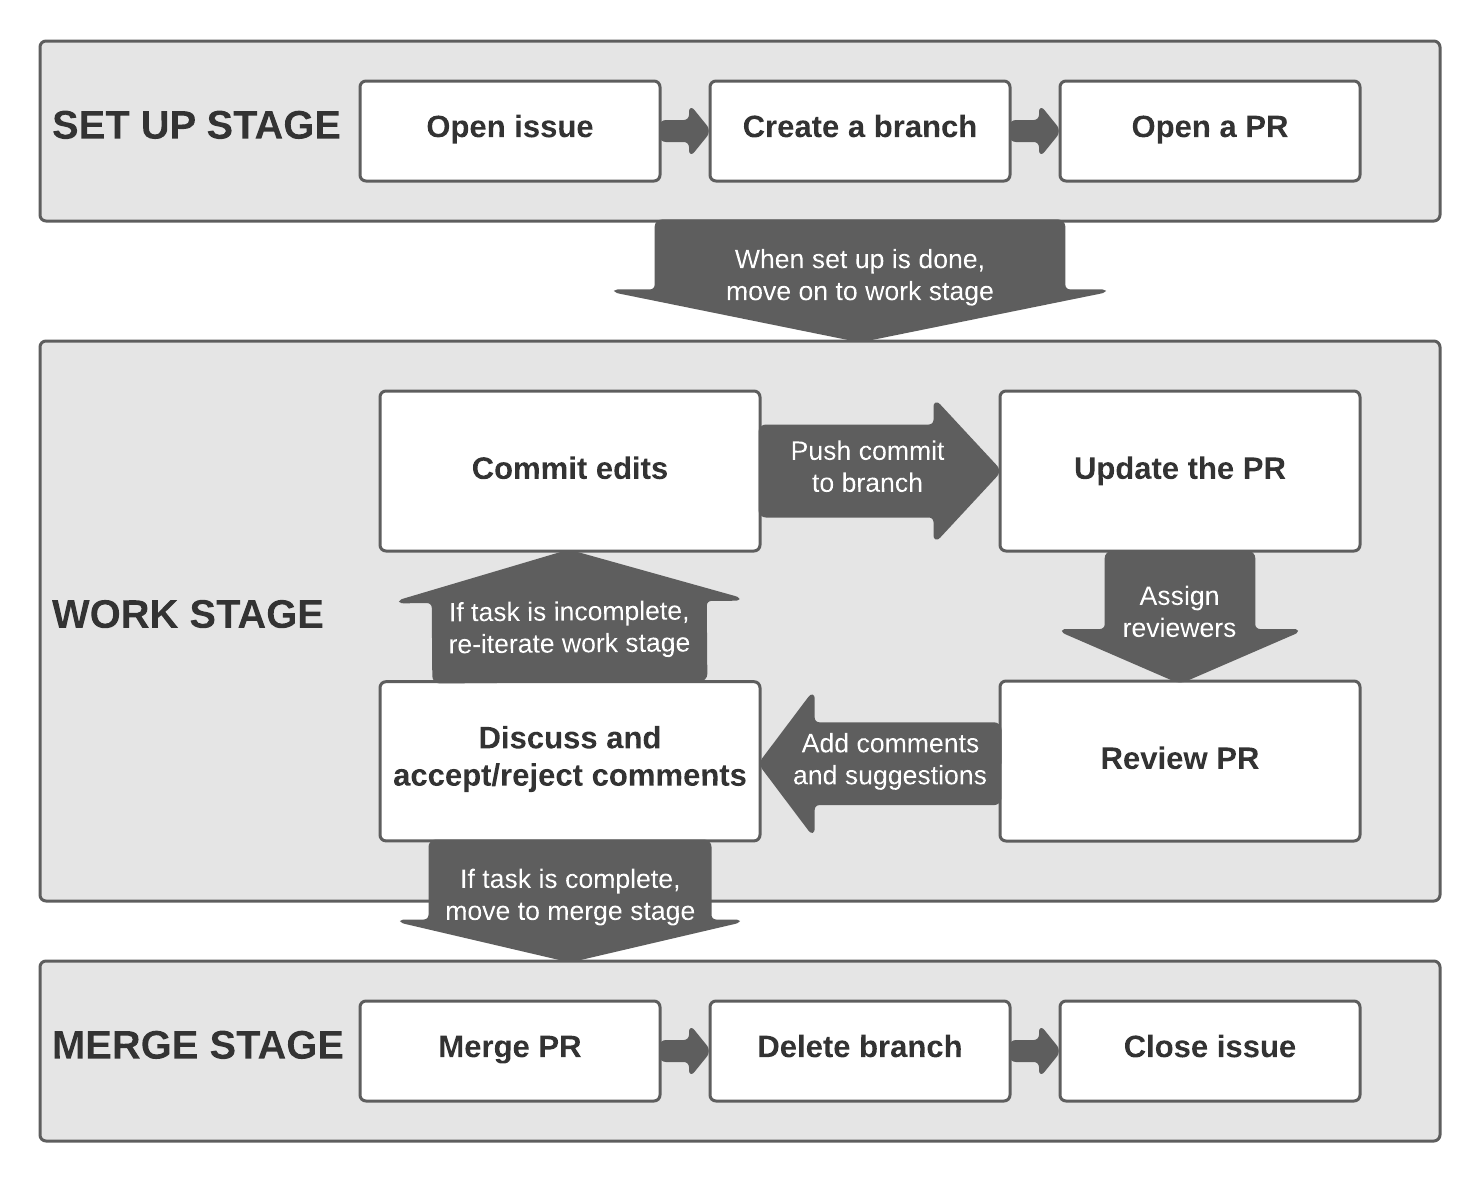
\includegraphics[width=\textwidth]{./img/branch-pr-merge-cycle.png}
		\end{figure}

	\end{columns}
\end{frame}

\begin{frame}
	\frametitle{Stage: The set up stage}

	\huge\centering \textbf{SET UP STAGE}

\end{frame}


\begin{frame}
	\frametitle{Stage: The set up stage}
	\begin{columns}[c]

		\column{.35\textwidth} % Left column and width

		\Large \textbf{The set up stage:}
		\vspace{1em}
		\normalsize

		\begin{itemize}
			\setlength\itemsep{1em}
			\item Document the task you will work on
			\item Create a space in your repo to work on the task
		\end{itemize}

		\column{.65\textwidth} % Right column and width
		\vspace{-.75cm}
		\begin{figure}
			\centering
			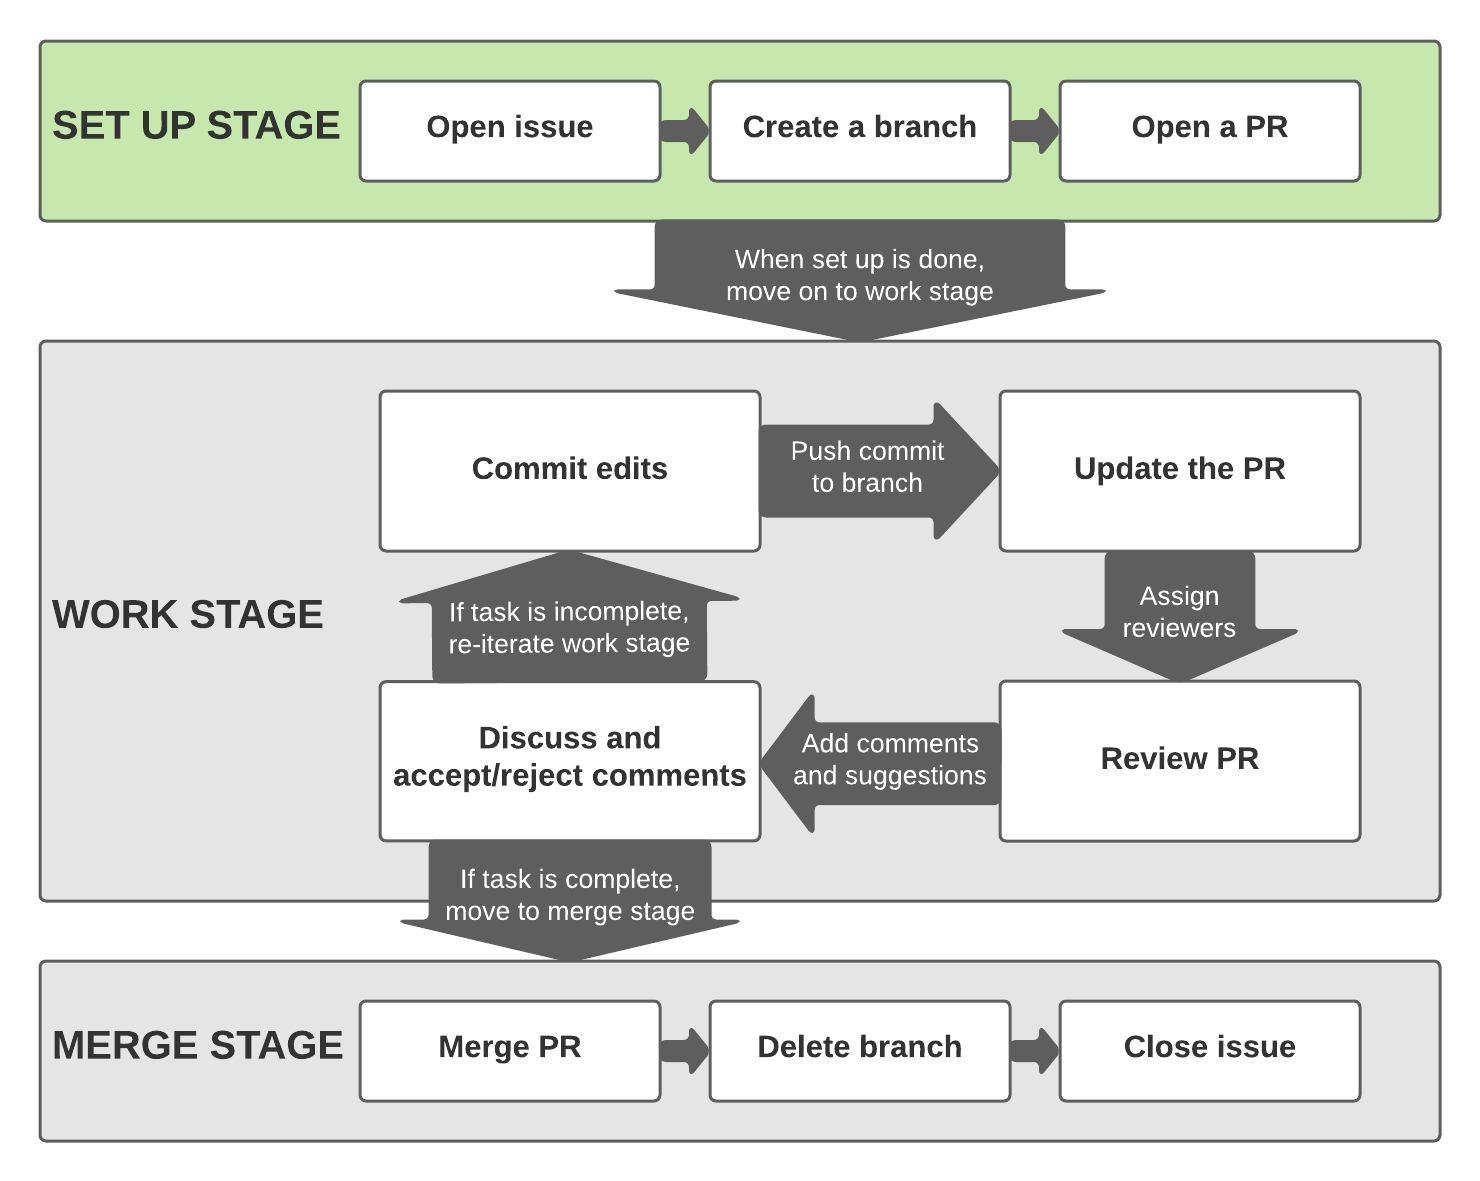
\includegraphics[width=\textwidth]{./img/branch-pr-merge-cycle-S1.png}
		\end{figure}

	\end{columns}
\end{frame}


\begin{frame}
	\frametitle{Step: Create an issue}
	\begin{columns}[c]

		\column{.35\textwidth} % Left column and width
		\begin{itemize}
			\setlength\itemsep{.5em}
			\item Issues are a great way to document what tasks need to be done
			\item They allow other team members to provide input
			on how to solve the task
			\item No need to open an issue for tasks
			that will be done immediately and
			don't require a place to document related discussions
		\end{itemize}

		\column{.65\textwidth} % Right column and width
		\vspace{-.75cm}
		\begin{figure}
			\centering
			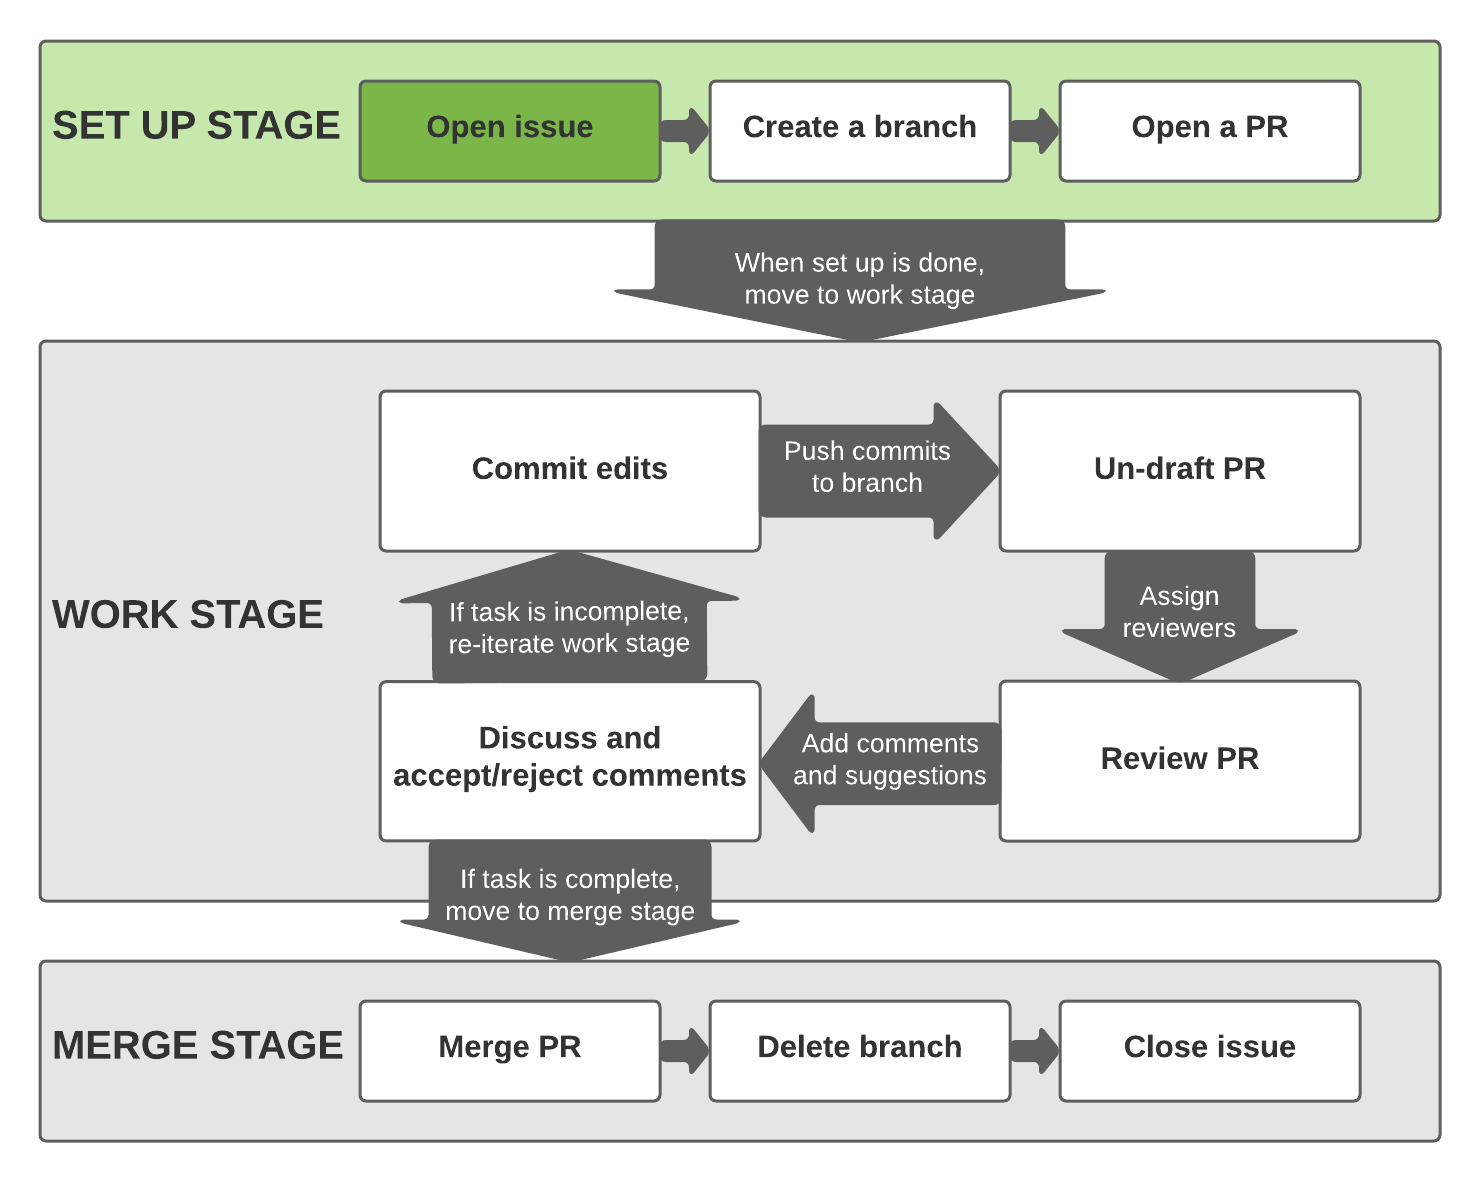
\includegraphics[width=\textwidth]{./img/branch-pr-merge-cycle-S1-1.png}
		\end{figure}

	\end{columns}
\end{frame}

\begin{frame}
	\frametitle{Create an issue}
	\begin{columns}[c]

		\column{.55\textwidth} % Right column and width
		\vspace{-.5cm}
		\begin{figure}
			\centering
			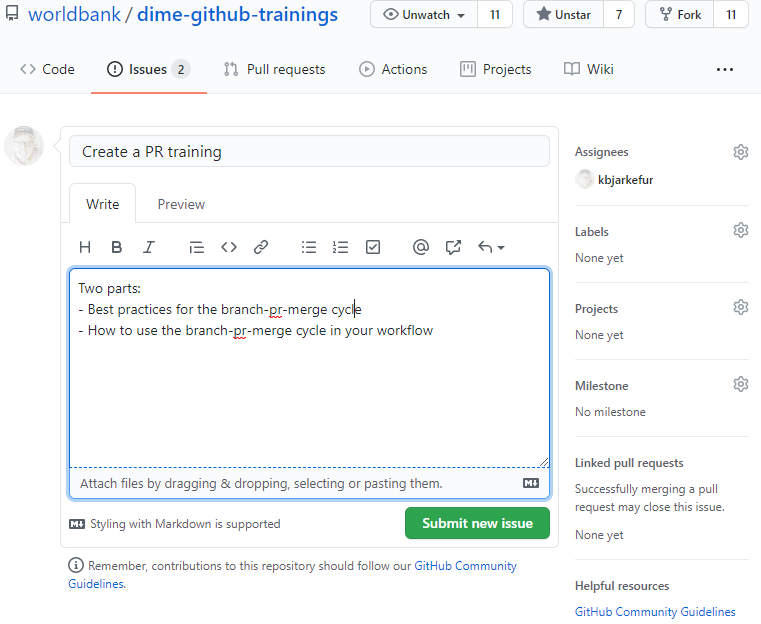
\includegraphics[width=\textwidth]{./img/create-issue-1.png}
		\end{figure}

		\column{.45\textwidth} % Left column and width

		\begin{itemize}
			\setlength\itemsep{.5em}
			\item Click the issues tab and then \texttt{New Issue}
			\item Document the task and/or ask the rest of the team of input
			\item Assign yourself or someone else to complete the task
			\item Add labels to facilitate future searches
			\item This is a far superior way to document tasks
			compared to emails or in-person meetings!
		\end{itemize}

	\end{columns}
\end{frame}

\begin{frame}
	\frametitle{Browse an issue}
	\begin{columns}[c]

		\column{.55\textwidth} % Right column and width
		\vspace{-.5cm}
		\begin{figure}
			\centering
			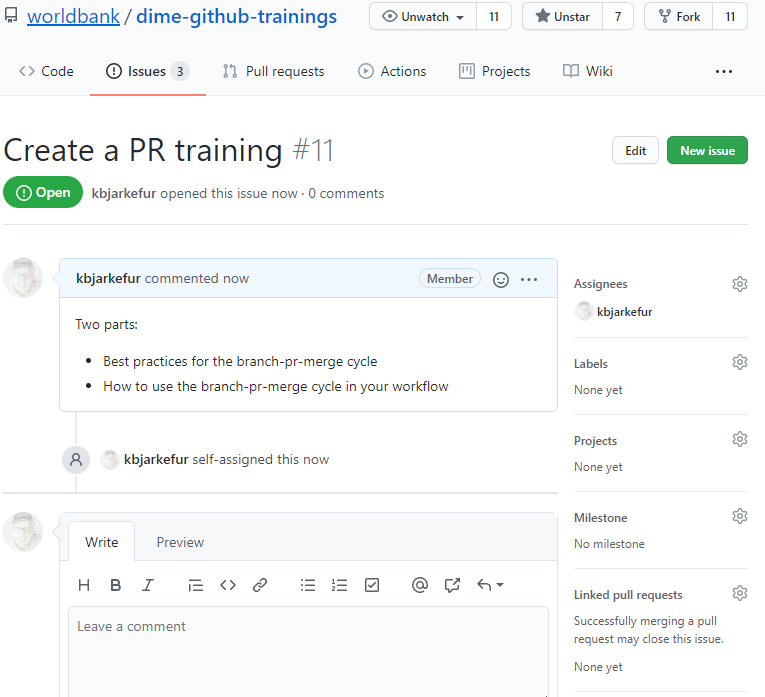
\includegraphics[width=\textwidth]{./img/create-issue-2.png}
		\end{figure}

		\column{.45\textwidth} % Left column and width

		\begin{itemize}
			\setlength\itemsep{1em}
			\item Take note of the issue number
			(also found in end of issue URL)
			so you can refer to it
			\item Anyone can use the comment field to provide input
			\item You can update assignees and/or labels
			\item Even when closed,
			this issue may be browsed by future team members
		\end{itemize}

	\end{columns}
\end{frame}

\begin{frame}
	\frametitle{Create a branch}
	\begin{columns}[c]

		\column{.35\textwidth} % Left column and width
		\begin{itemize}
			\setlength\itemsep{.5em}
			\item Create branch on GitHub.com
			\hyperlink{new-branch}{\beamergotobutton{Step-by-step}}
			\item We create a branch to have a space
			where work on this task does not interfere
			with work on other tasks
			\item Name the branch after the task and
			add the issue number as suffix - for example:
			\texttt{pr-training-11}
		\end{itemize}

		\column{.65\textwidth} % Right column and width
		\vspace{-.75cm}
		\begin{figure}
			\centering
			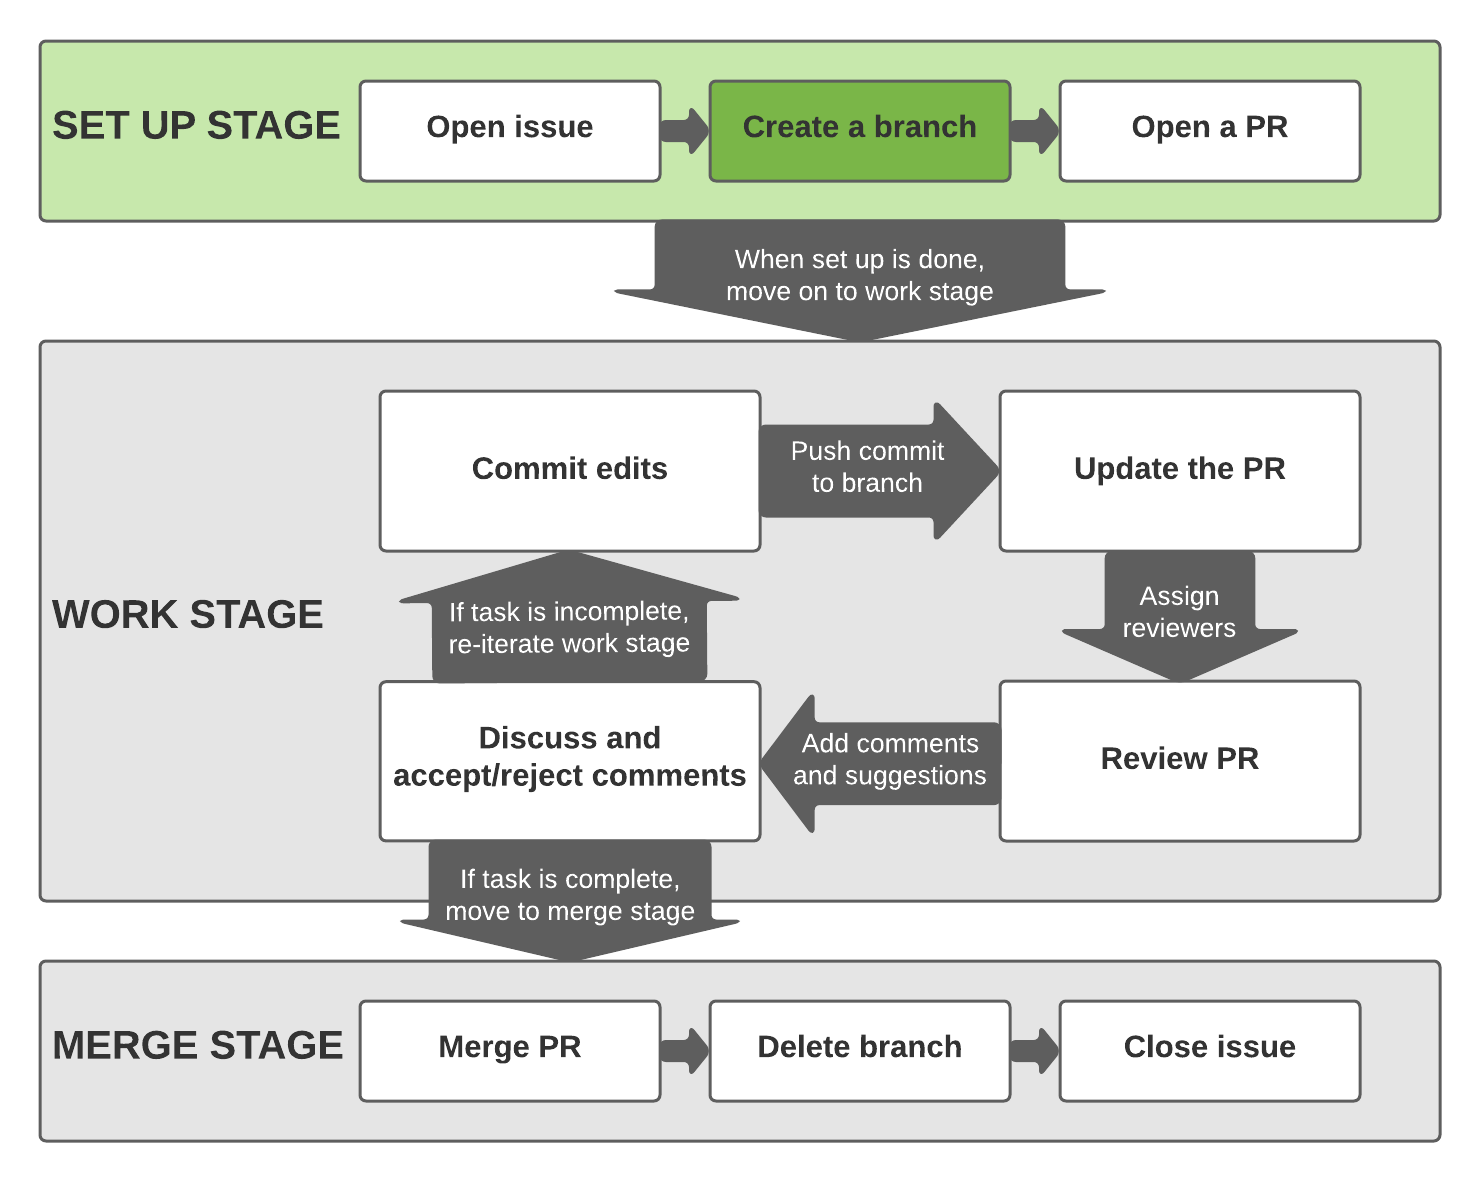
\includegraphics[width=\textwidth]{./img/branch-pr-merge-cycle-S1-2.png}
		\end{figure}

	\end{columns}
\end{frame}

\begin{frame}
	\frametitle{Open the PR}
	\begin{columns}[c]

		\column{.35\textwidth} % Left column and width
		\begin{itemize}
			\setlength\itemsep{1em}
			\item Create a PR \textbf{before} you start working
			- this creates a space on GitHub
			where the progress of this task can be followed
			\item Create a \textit{``draft PR''} for work in progress
			\item Reference branch name in PR name
		\end{itemize}

		\column{.65\textwidth} % Right column and width
		\vspace{-.75cm}
		\begin{figure}
			\centering
			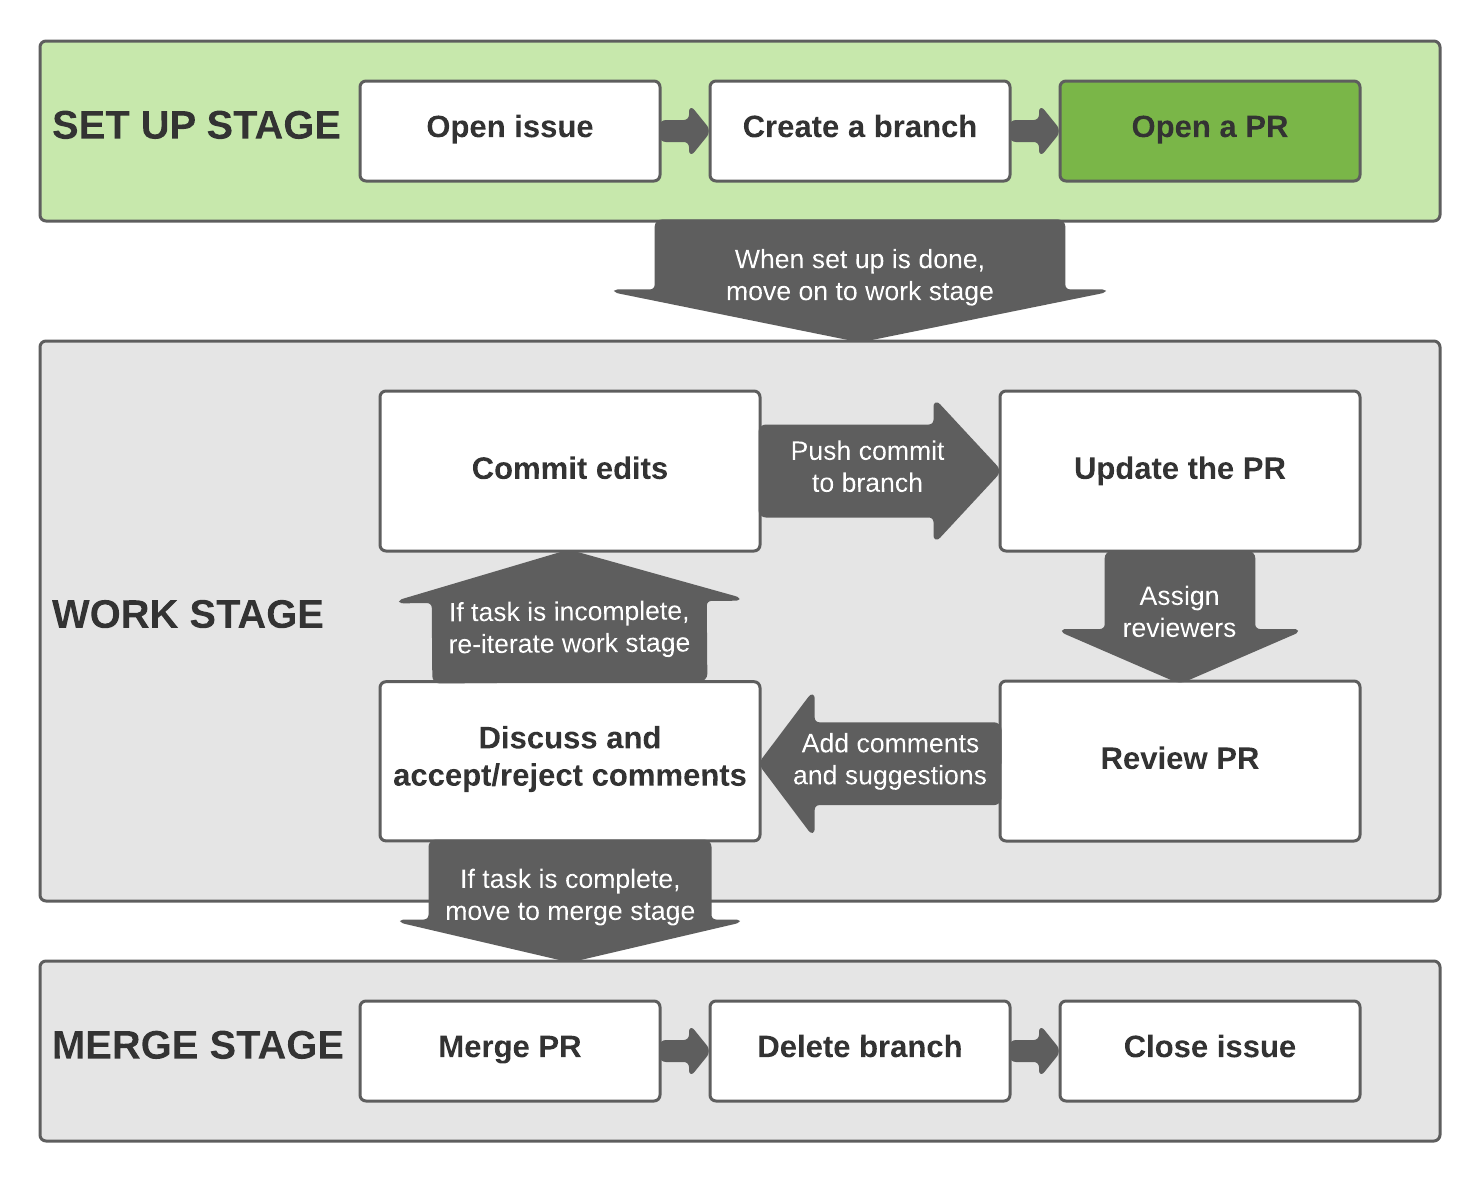
\includegraphics[width=\textwidth]{./img/branch-pr-merge-cycle-S1-3.png}
		\end{figure}

	\end{columns}
\end{frame}

\begin{frame}
	\frametitle{Create a PR}
	\begin{columns}[c]

		\column{.53\textwidth} % Right column and width
		\vspace{-.5cm}
		\begin{figure}
			\centering
			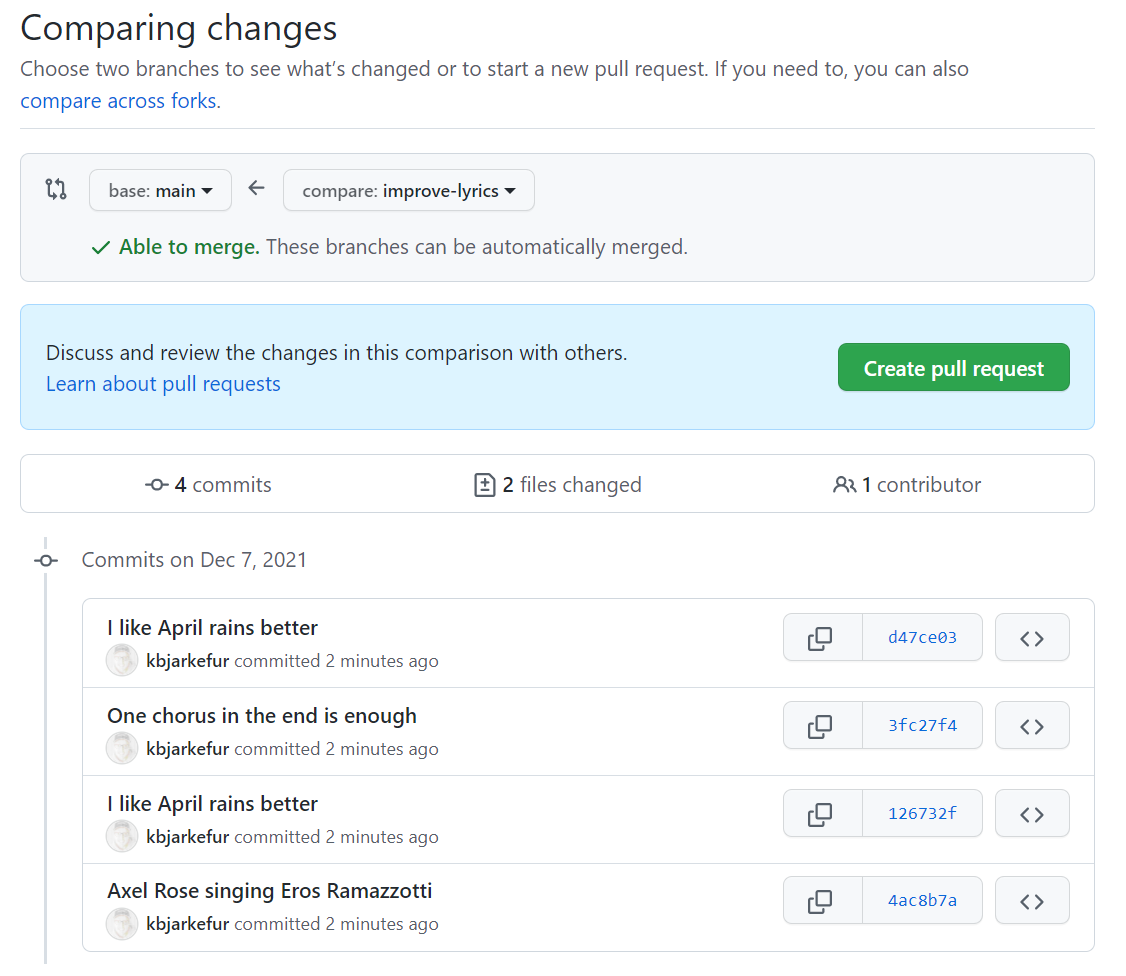
\includegraphics[width=\textwidth]{./img/create-pr-0.png}
		\end{figure}

		\column{.47\textwidth} % Left column and width
		Recap of PR creation best practices:
		\vspace{.5cm}
		\begin{itemize}
			\setlength\itemsep{.5em}
			\item Go to the \textit{``Pull request''} tab
			\item Make sure that you are comparing the correct branches
			\item Always browse the commits and
			the files changes before opening the PR
			\item You need at least one commit
			- Create/edit a README describing the task
		\end{itemize}

	\end{columns}
\end{frame}

\begin{frame}
	\frametitle{Create a draft PR}
	\begin{columns}[c]

		\column{.53\textwidth} % Right column and width
		\vspace{-.5cm}
		\begin{figure}
			\centering
			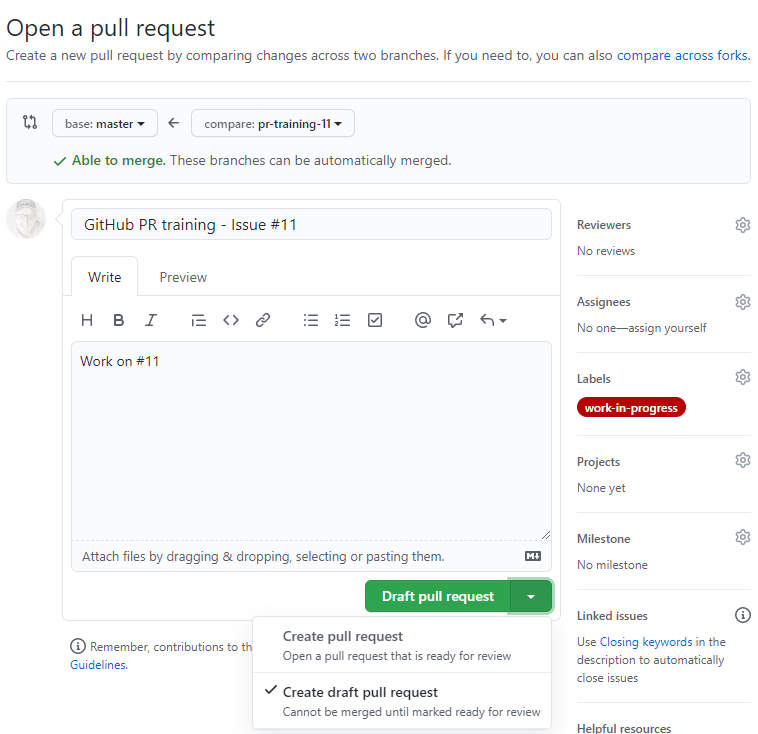
\includegraphics[width=\textwidth]{./img/create-pr-1.png}
		\end{figure}

		\column{.47\textwidth} % Left column and width

		\begin{itemize}
			\setlength\itemsep{.5em}
			\item Give the PR a name associated with
			the branch name but more descriptive
			\item Add \texttt{\#11} in the description
			to create a hyper link to issue
			- add \texttt{work-in-progress} label
			\item Click the arrow on the green button and
			select \textit{Create draft pull request}
			\item A PR cannot be merged while in draft status
			- signals work in progress
		\end{itemize}

	\end{columns}
\end{frame}

\begin{frame}
	\frametitle{Browse draft PR}
	\begin{columns}[c]

		\column{.6\textwidth} % Right column and width
		\vspace{-.5cm}
		\begin{figure}
			\centering
			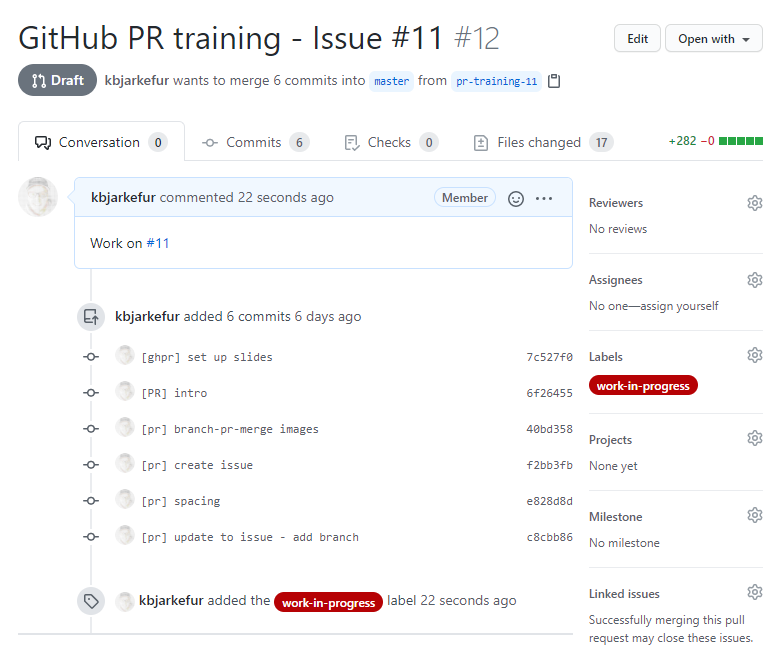
\includegraphics[width=\textwidth]{./img/create-pr-2.png}
		\end{figure}

		\column{.4\textwidth} % Left column and width

		\begin{itemize}
			\setlength\itemsep{1em}
			\item A draft PR has the color code gray
			\item You can follow someone's work here
			- but no one is required to review anything yet
			\item The author will eventually remove the draft status
			and ask for reviews
		\end{itemize}

	\end{columns}
\end{frame}

\begin{frame}
	\frametitle{Stage: The work stage}

	\huge\centering \textbf{WORK STAGE}

\end{frame}

\begin{frame}
	\frametitle{Stage: The work stage}
	\begin{columns}[c]

		\column{.35\textwidth} % Left column and width

		\Large \textbf{The work stage:}
		\vspace{.5em}
		\normalsize
		\begin{itemize}
			\setlength\itemsep{.5em}
			\item Most time will be spent in this stage
			\item Reviewing the code should be seen as a step
			as important as writing it
			\item This stage will be repeated until
			the team agrees on the quality of the code
		\end{itemize}

		\column{.65\textwidth} % Right column and width
		\vspace{-.75cm}
		\begin{figure}
			\centering
			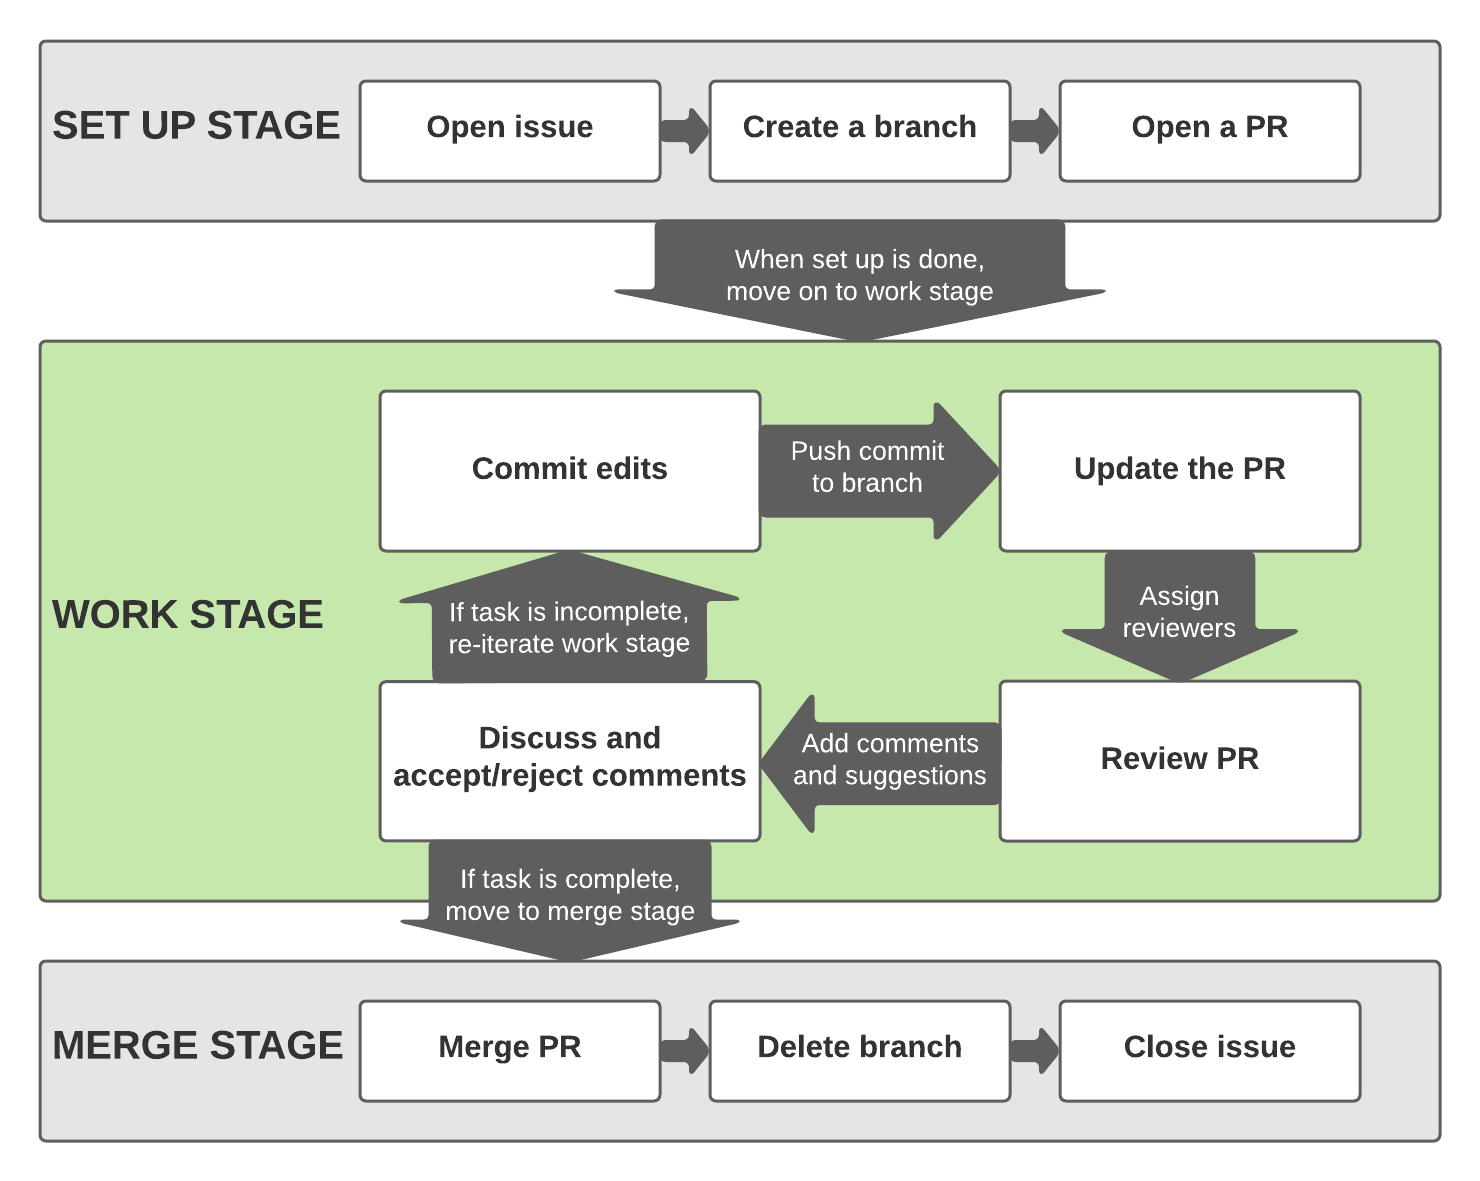
\includegraphics[width=\textwidth]{./img/branch-pr-merge-cycle-S2.png}
		\end{figure}

	\end{columns}
\end{frame}

\begin{frame}
	\frametitle{Make commits}
	\begin{columns}[c]

		\column{.35\textwidth} % Left column and width
		\begin{itemize}
			\setlength\itemsep{1em}
			\item The author commits edits as usual
			\item The draft PR will be updated as
			more commits are pushed to the branch
			\item Keep pushing commits until
			the first implementation of the task is complete
		\end{itemize}

		\column{.65\textwidth} % Right column and width
		\vspace{-.75cm}
		\begin{figure}
			\centering
			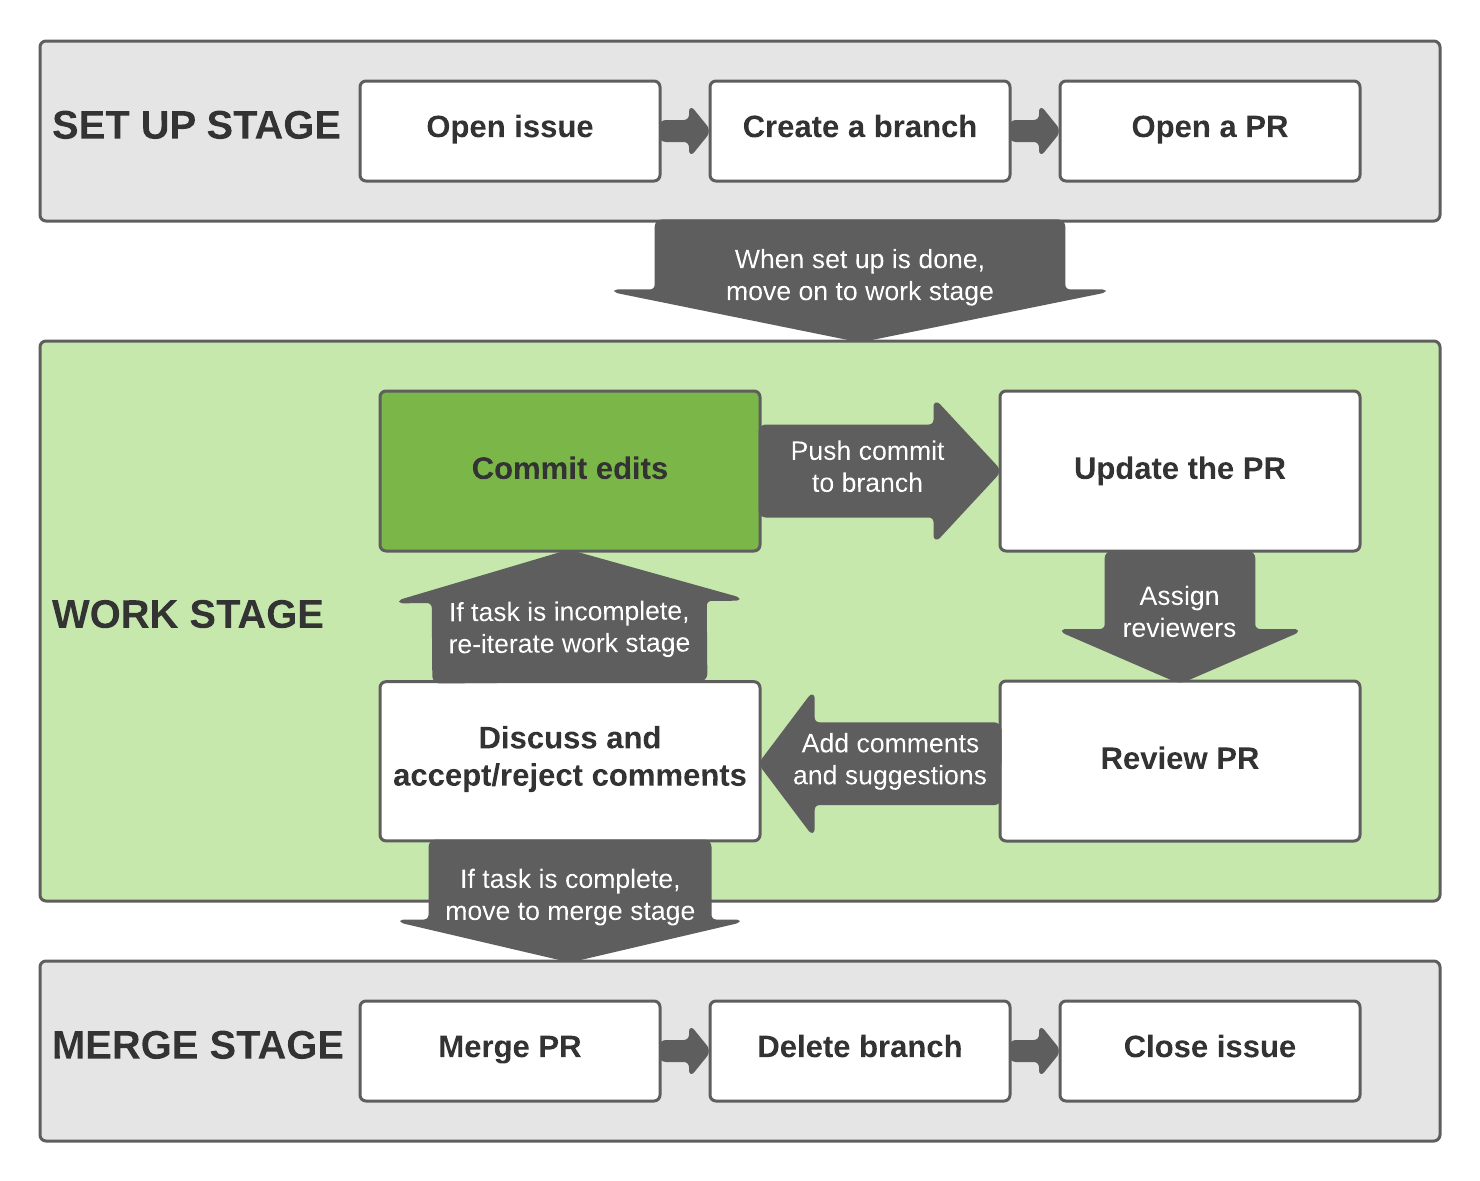
\includegraphics[width=\textwidth]{./img/branch-pr-merge-cycle-S2-1.png}
		\end{figure}

	\end{columns}
\end{frame}

\begin{frame}
	\frametitle{Un-draft the PR}
	\begin{columns}[c]

		\column{.35\textwidth} % Left column and width
		\begin{itemize}
			\setlength\itemsep{1em}
			\item Remove the draft status from the PR
			\item Assign one or several people to review your PR
			\item Notify the reviewer(s) using email
			or slack as GitHub notifications may be muted
		\end{itemize}

		\column{.65\textwidth} % Right column and width
		\vspace{-.75cm}
		\begin{figure}
			\centering
			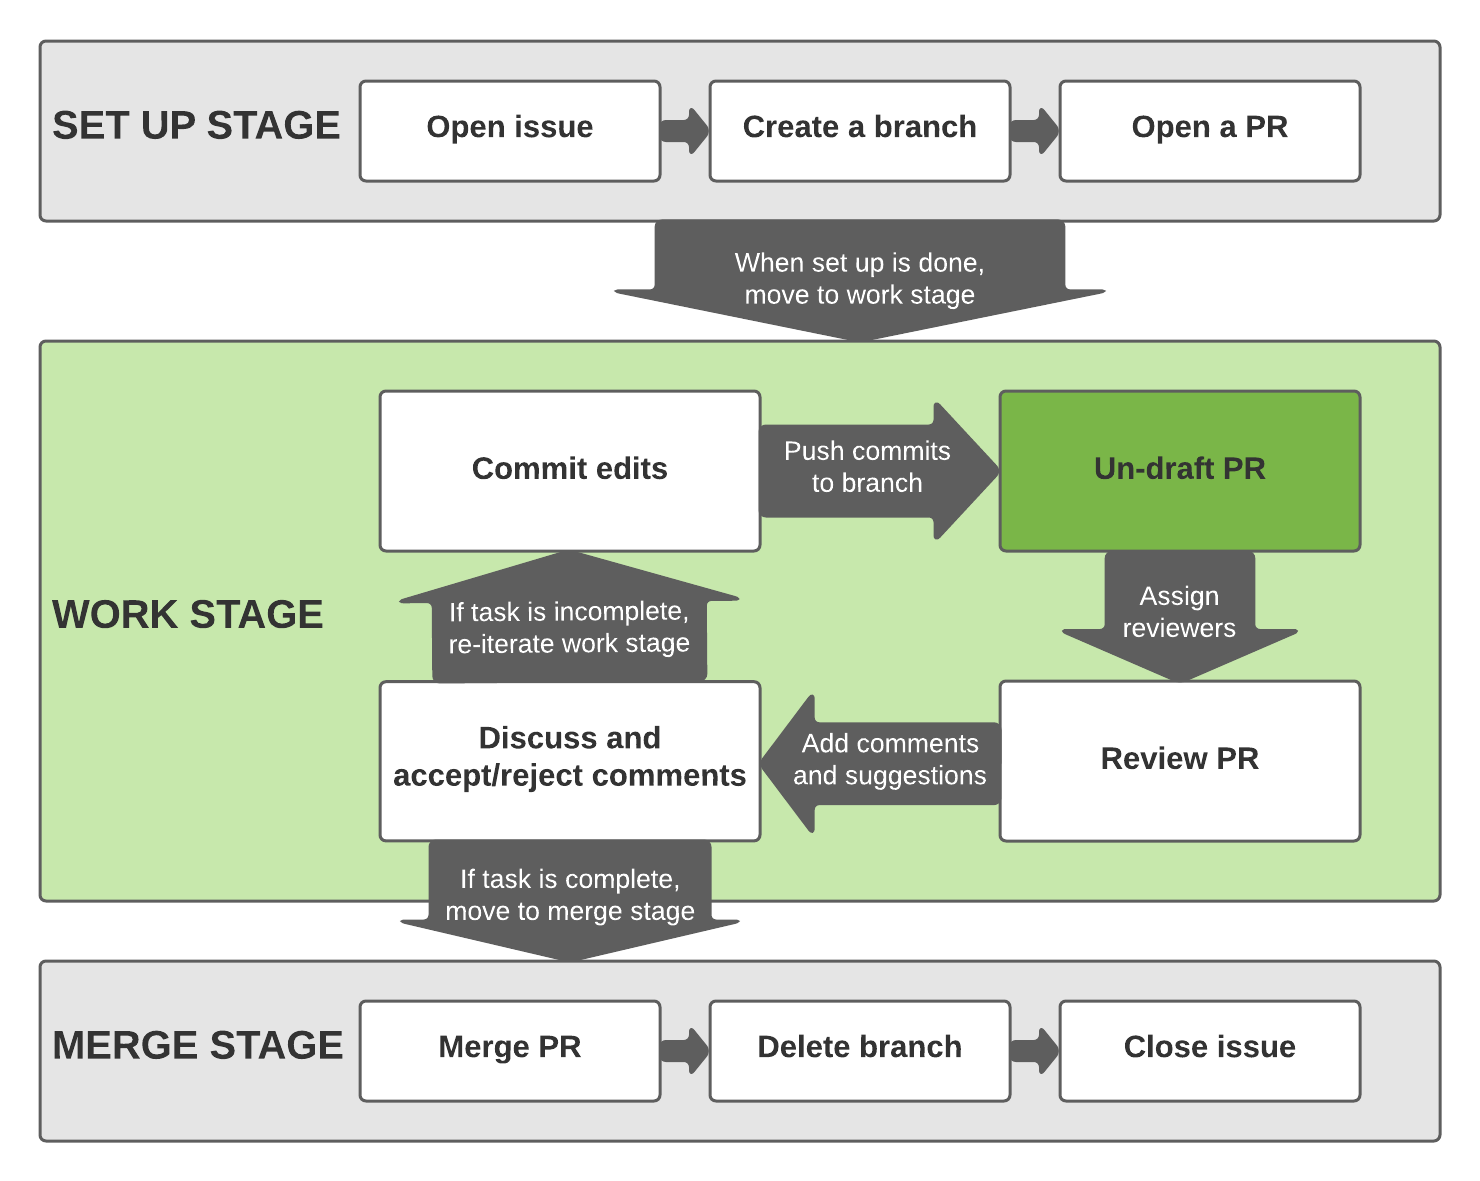
\includegraphics[width=\textwidth]{./img/branch-pr-merge-cycle-S2-2.png}
		\end{figure}

	\end{columns}
\end{frame}

\begin{frame}
	\frametitle{Un-draft the PR}
	\begin{columns}[c]

	\column{.6\textwidth} % Right column and width
	\vspace{-.75cm}
	\begin{figure}
		\centering
		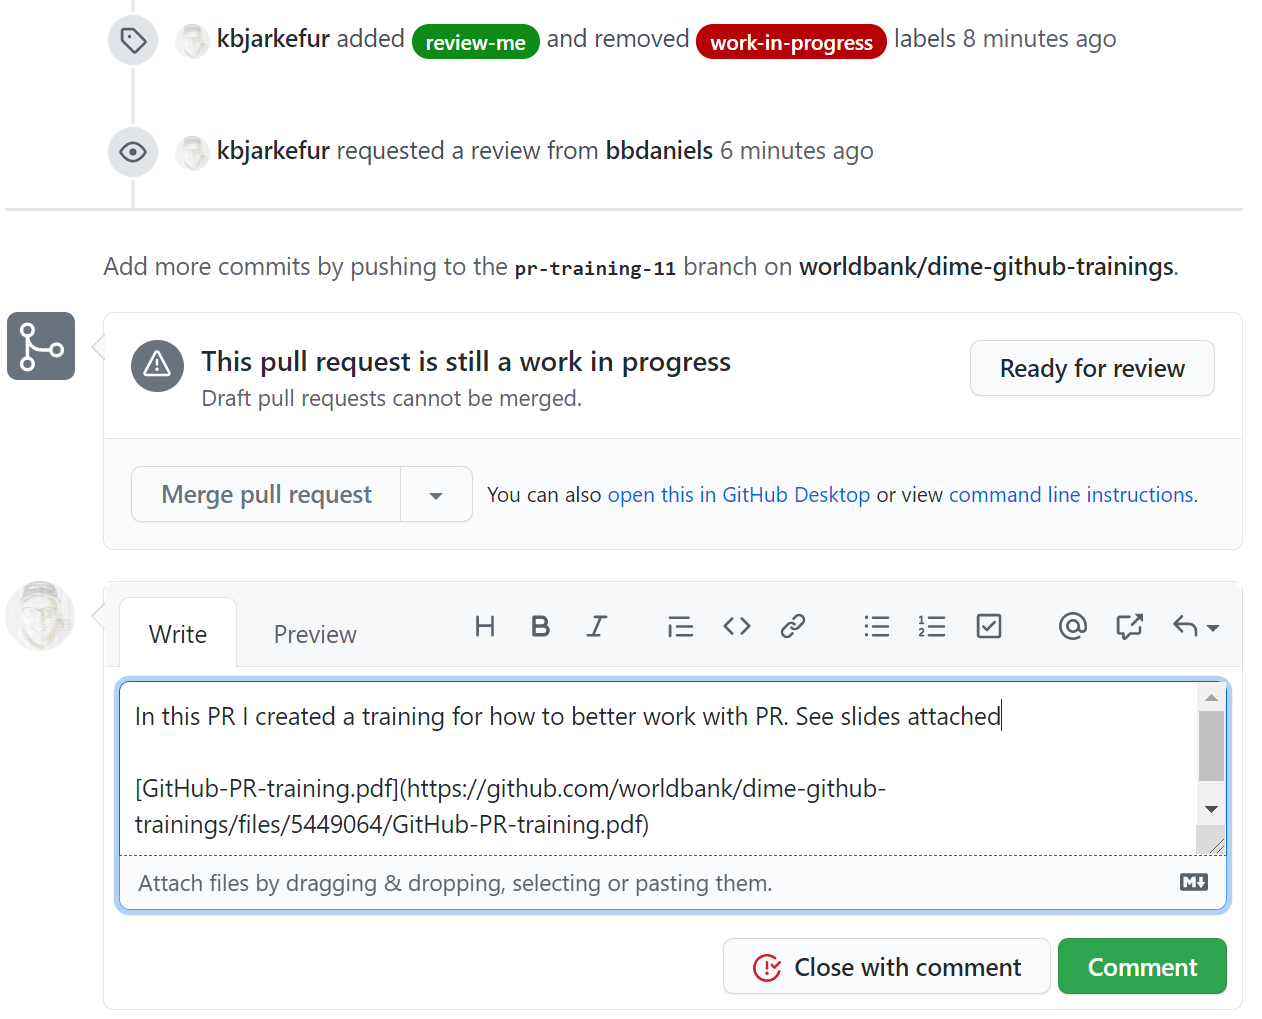
\includegraphics[width=\textwidth]{./img/undraft-pr.png}
	\end{figure}

	\column{.4\textwidth} % Left column and width
	\begin{itemize}
		\setlength\itemsep{1em}
		\item Replace the \textit{work-in-progress} label
		with \textit{review-me}
		\item Document what has been implemented in the branch
		\item Click \textit{``Ready for review''} to remove draft status
	\end{itemize}

\end{columns}
\end{frame}

\begin{frame}
	\frametitle{Review the PR}
	\begin{columns}[c]

		\column{.35\textwidth} % Left column and width
		\begin{itemize}
			\setlength\itemsep{1em}
			\item This step is incredibly important for high-quality code
			\item Use the PR to review code edits
			in the \textit{file changes} tab
			\item The reviewer adds code suggestions and comments
		\end{itemize}

		\column{.65\textwidth} % Right column and width
		\vspace{-.75cm}
		\begin{figure}
			\centering
			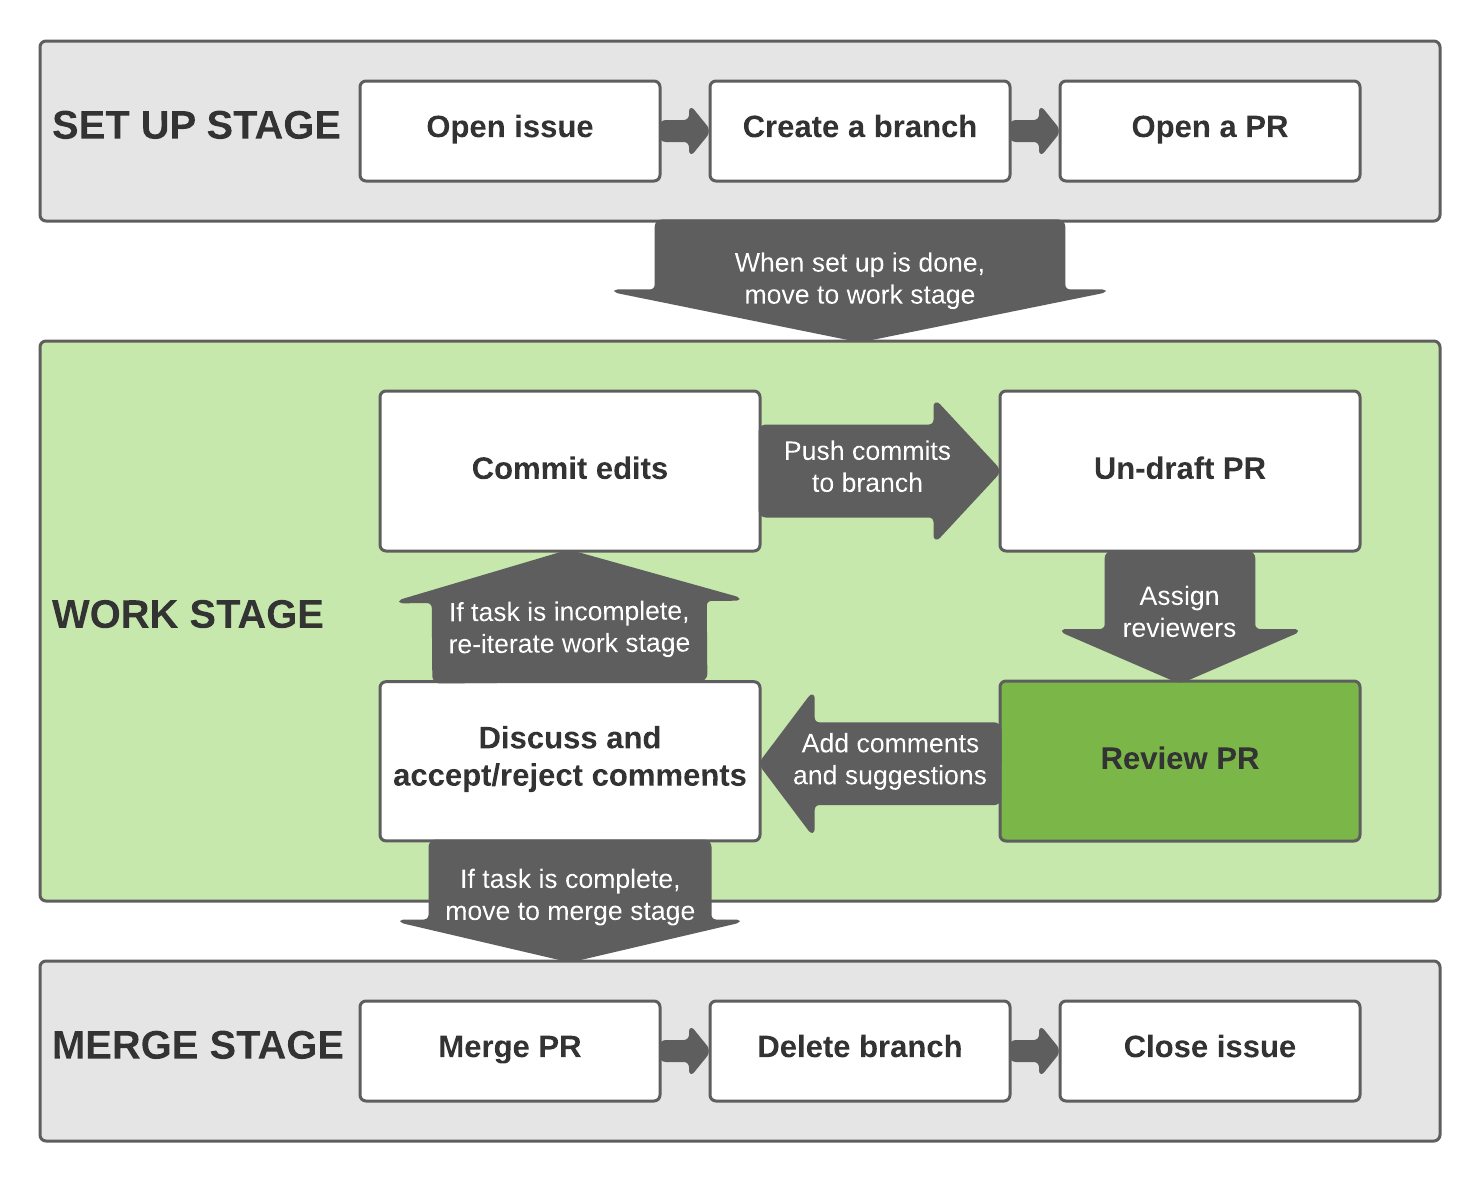
\includegraphics[width=\textwidth]{./img/branch-pr-merge-cycle-S2-3.png}
		\end{figure}

	\end{columns}
\end{frame}

\begin{frame}
	\frametitle{Review the PR}
	\begin{columns}[c]

		\column{.65\textwidth} % Right column and width
		\vspace{-.75cm}
		\begin{figure}
			\centering
			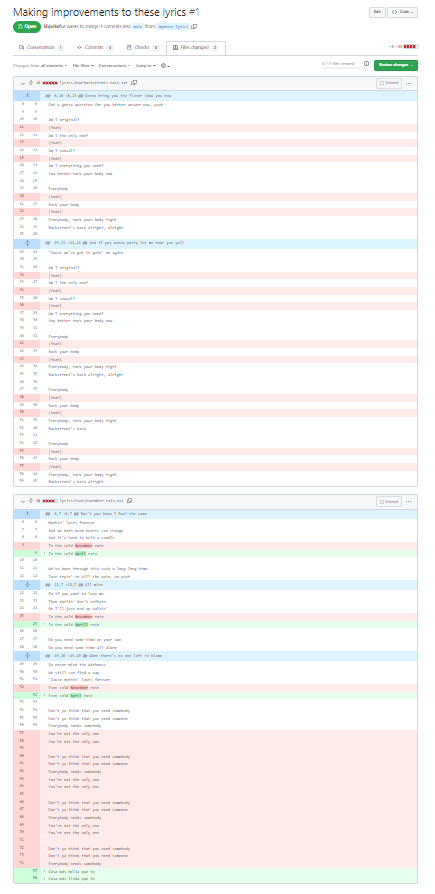
\includegraphics[width=\textwidth]{./img/review-1.png}
		\end{figure}

		\column{.35\textwidth} % Left column and width
		\begin{itemize}
			\setlength\itemsep{2em}
			\item When reviewing a PR,
			always start by reading what the author or anyone else
			have written in the \textit{``Conversation"} tab
			\item Then go to the \textit{``Files changed''} tab
			- this is where you will review the new content of the files
		\end{itemize}

	\end{columns}
\end{frame}


\begin{frame}
	\frametitle{Line comments}
	\begin{columns}[c]

		\column{.50\textwidth} % Right column and width
		\vspace{-.6cm}
		\begin{figure}
			\centering
			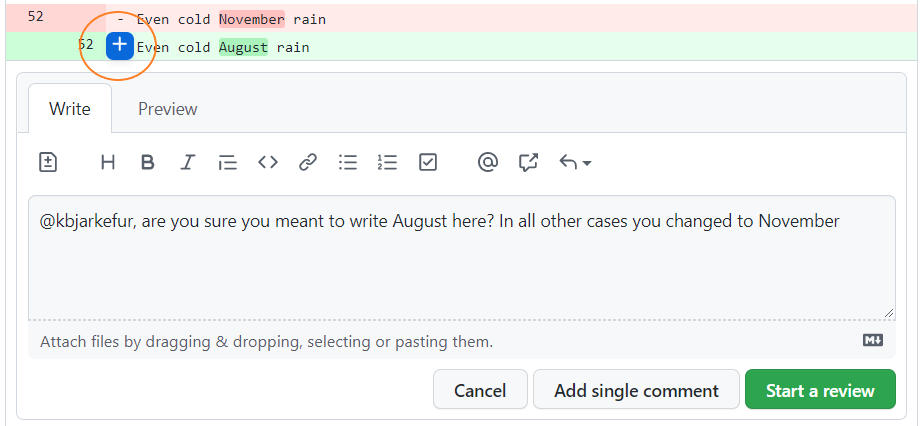
\includegraphics[width=\textwidth]{./img/line-comment-1.png}
		\end{figure}
		\vspace{-.3cm}
		\begin{figure}
			\centering
			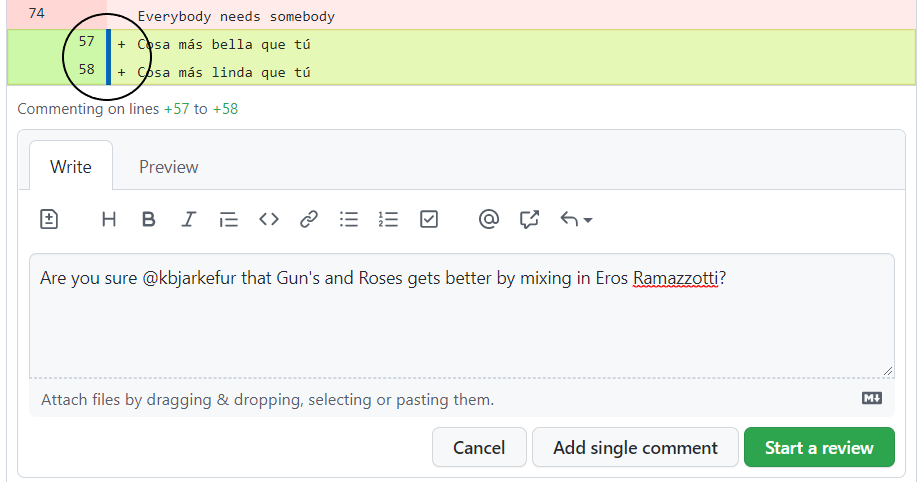
\includegraphics[width=\textwidth]{./img/line-comment-2.png}
		\end{figure}

		\column{.50\textwidth} % Left column and width
		\begin{itemize}
			\setlength\itemsep{.74em}
			\item Make comments on specific lines of as much as possible
			- line comments are much easier to keep track of
			\item Click plus sign in blue circle to comment on a line
			\item Hold shift when click and drag mouse to comment multiple lines
		\end{itemize}

	\end{columns}
\end{frame}

\begin{frame}
	\frametitle{Line suggestions}
	\begin{columns}[c]

		\column{.50\textwidth} % Right column and width
		\vspace{-.6cm}
		\begin{figure}
			\centering
			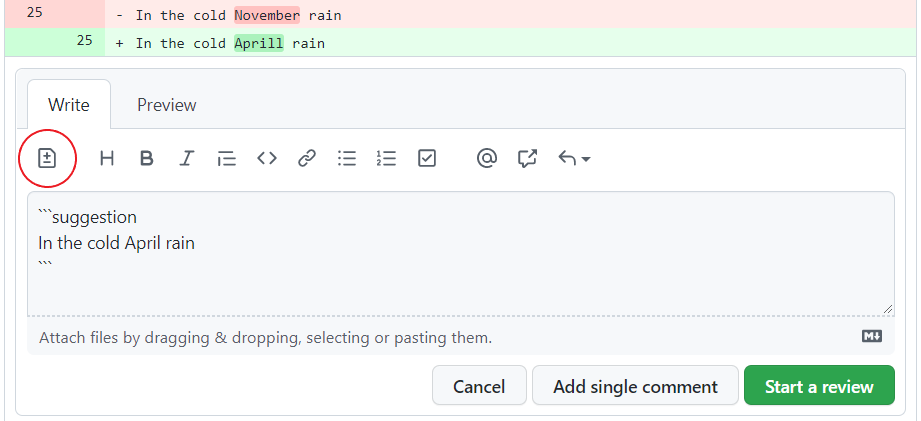
\includegraphics[width=\textwidth]{./img/suggestion-1.png}
		\end{figure}
		\vspace{-.3cm}
		\begin{figure}
			\centering
			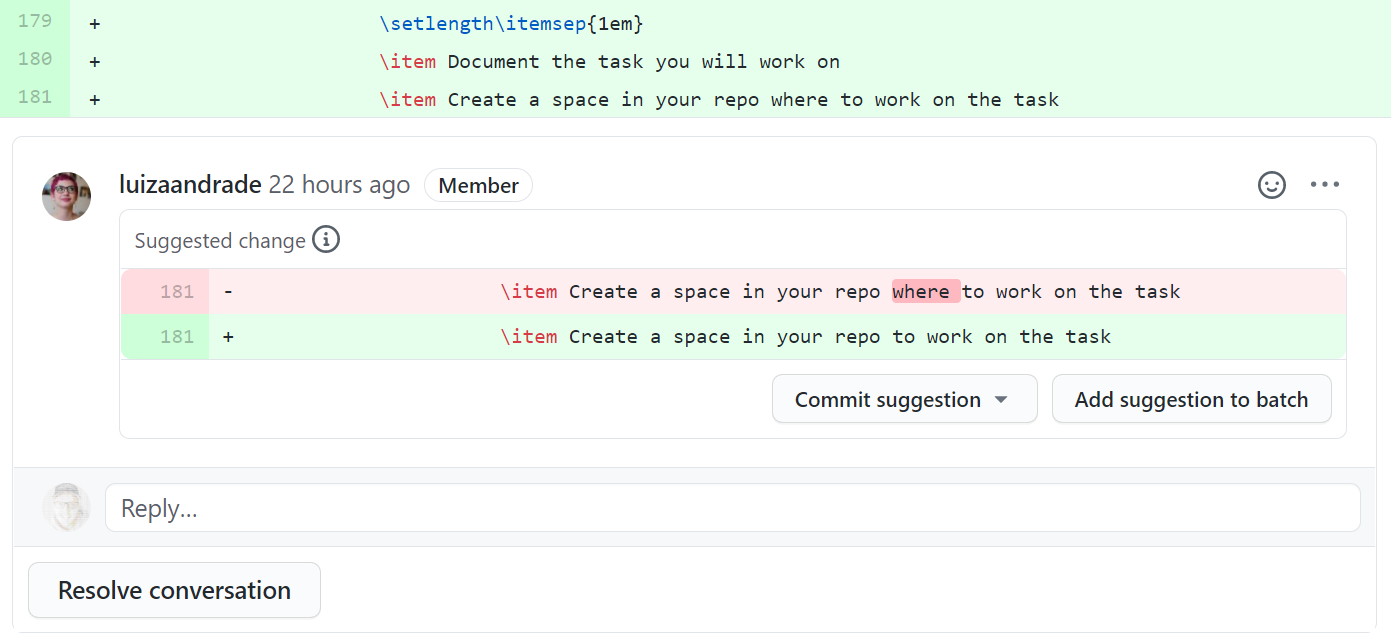
\includegraphics[width=\textwidth]{./img/suggestion-2.png}
		\end{figure}

		\column{.50\textwidth} % Left column and width
		\begin{itemize}
			\setlength\itemsep{.74em}
			\item You can also suggest an edit directly to the code
			if the edit is not too big
			\item Click the suggestion button (red circle), and edit the line
			\item The author will then see the edit that you are suggesting
			\item Can be done in multi line comments too
		\end{itemize}

	\end{columns}
\end{frame}

\begin{frame}
	\frametitle{Overall comments}
	\begin{columns}[c]

		\column{.6\textwidth} % Right column and width
		\vspace{-.75cm}
		\begin{figure}
			\centering
			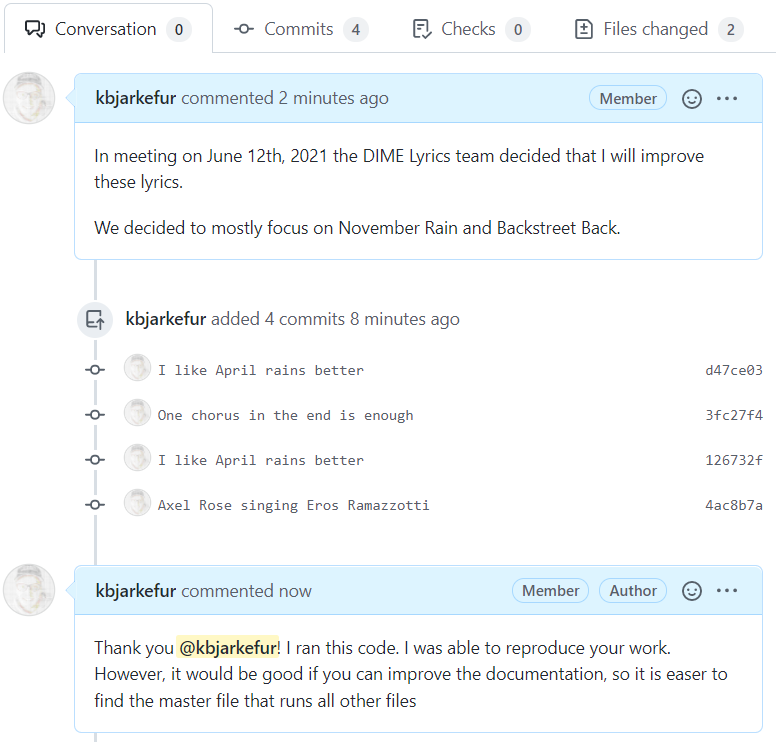
\includegraphics[width=\textwidth]{./img/pr-comment.png}
		\end{figure}

		\column{.4\textwidth} % Left column and width
		\begin{itemize}
			\setlength\itemsep{1em}
			\item Make overall comments and comments
			that cannot be done to a specific section of the code
			in thread in the \textit{``Conversation''} tab
			\item Suggestions are also listed here
			\item Tag the author so they get a notification
			that someone have reviewed the PR
		\end{itemize}

	\end{columns}
\end{frame}

\begin{frame}
	\frametitle{Discuss and accept/reject}
	\begin{columns}[c]

		\column{.35\textwidth} % Left column and width
		\begin{itemize}
			\setlength\itemsep{1em}
			\item The author discusses, accepts or rejects suggestions
			and replies to comments
			\item Then the author and the reviewers
			(and anyone else in the project team)
			come together and decide if the task is complete or not
		\end{itemize}

		\column{.65\textwidth} % Right column and width
		\vspace{-.75cm}
		\begin{figure}
			\centering
			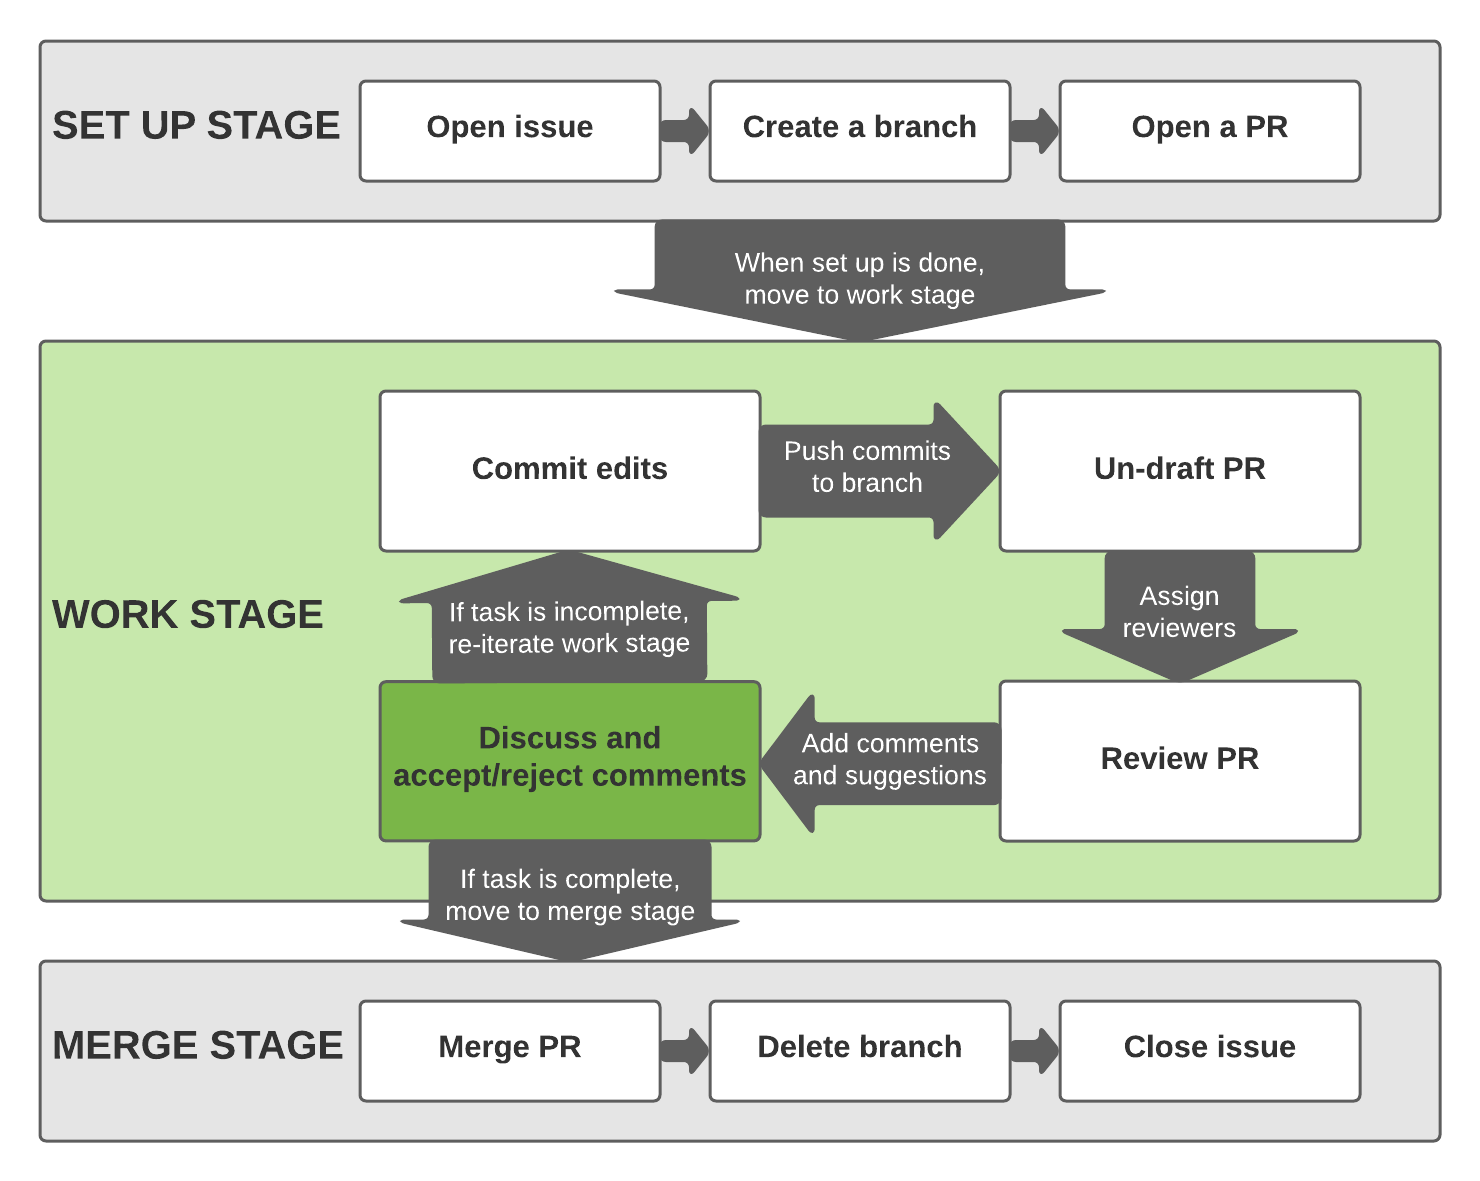
\includegraphics[width=\textwidth]{./img/branch-pr-merge-cycle-S2-4.png}
		\end{figure}

	\end{columns}
\end{frame}

\begin{frame}
	\frametitle{Review suggestion}
	\begin{columns}[c]

		\column{.5\textwidth} % Right column and width
		\vspace{-.75cm}
		\begin{figure}
			\centering
			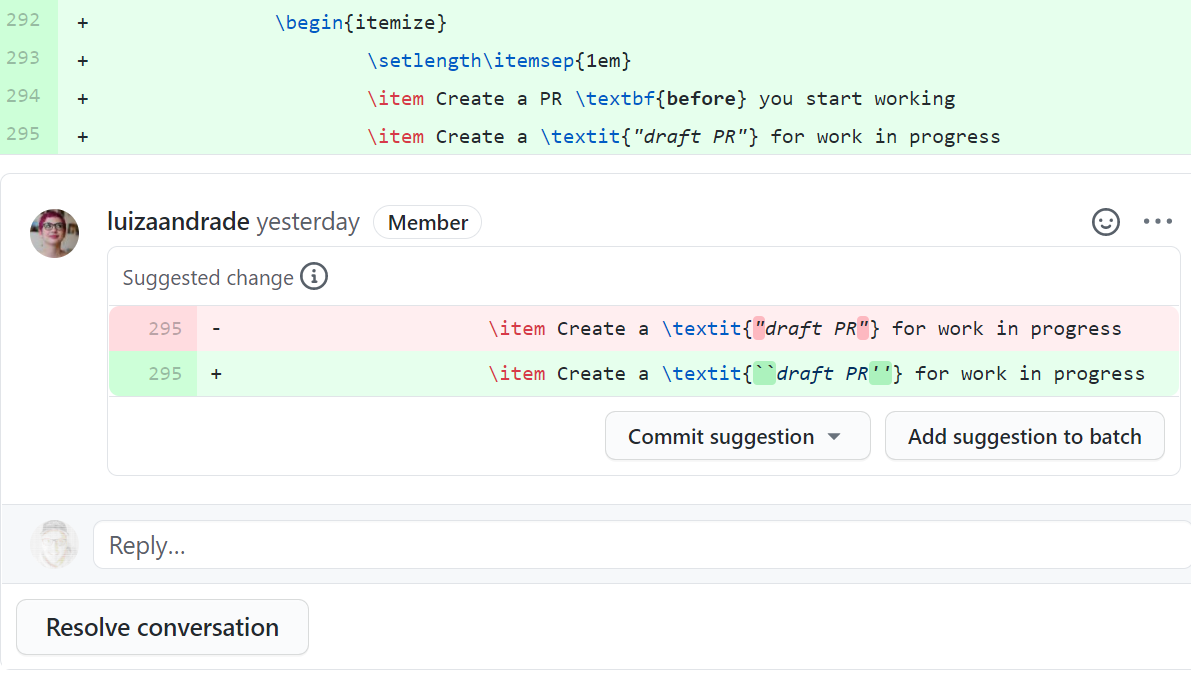
\includegraphics[width=\textwidth]{./img/review-suggestion-1.png}
		\end{figure}

		\column{.5\textwidth} % Left column and width
		\begin{itemize}
			\setlength\itemsep{1em}
			\item Start by going over the suggestions as they tend to be quick
			\item Suggestions are ordered chronologically
			in the \textit{``Conversation''} tab and
			by line number in the \textit{``File changes''} tab
			\item Accept the suggestion with \textit{Commit Suggestion},
			ignore/delete it with \textit{Resolve conversation}
			or comment to ask for more information
		\end{itemize}

	\end{columns}
\end{frame}

\begin{frame}
	\frametitle{Review suggestion}
	\begin{columns}[c]

		\column{.35\textwidth} % Right column and width
		\begin{figure}
			\centering
			
\includegraphics[width=.6\textwidth]{./img/qa.png}
		\end{figure}

		\column{.65\textwidth} % Left column and width
		\begin{itemize}
			\setlength\itemsep{1em}
			\item Address all suggestions and comments
			until they are all answered
			\item If major work is still required,
			put the PR in draft status again and
			add back the \textit{work-in-progress} label and
			start over the work stage
			\item Once there are no more small or major comments
			or suggestions left to do,
			then move on to the merge stage
		\end{itemize}

	\end{columns}
\end{frame}


\begin{frame}
	\frametitle{Stage: The merge stage}

	\huge\centering \textbf{MERGE STAGE}

\end{frame}

\begin{frame}
	\frametitle{Stage: The merge stage}
	\begin{columns}[c]

		\column{.35\textwidth} % Left column and width

		\Large \textbf{The merge stage:}
		\vspace{1em}
		\normalsize
		\begin{itemize}
			\setlength\itemsep{.5em}
			\item Once the work stage is complete, the merge stage is quick
			\item Clean up the task and make sure it was properly documented
		\end{itemize}

		\column{.65\textwidth} % Right column and width
		\vspace{-.75cm}
		\begin{figure}
			\centering
			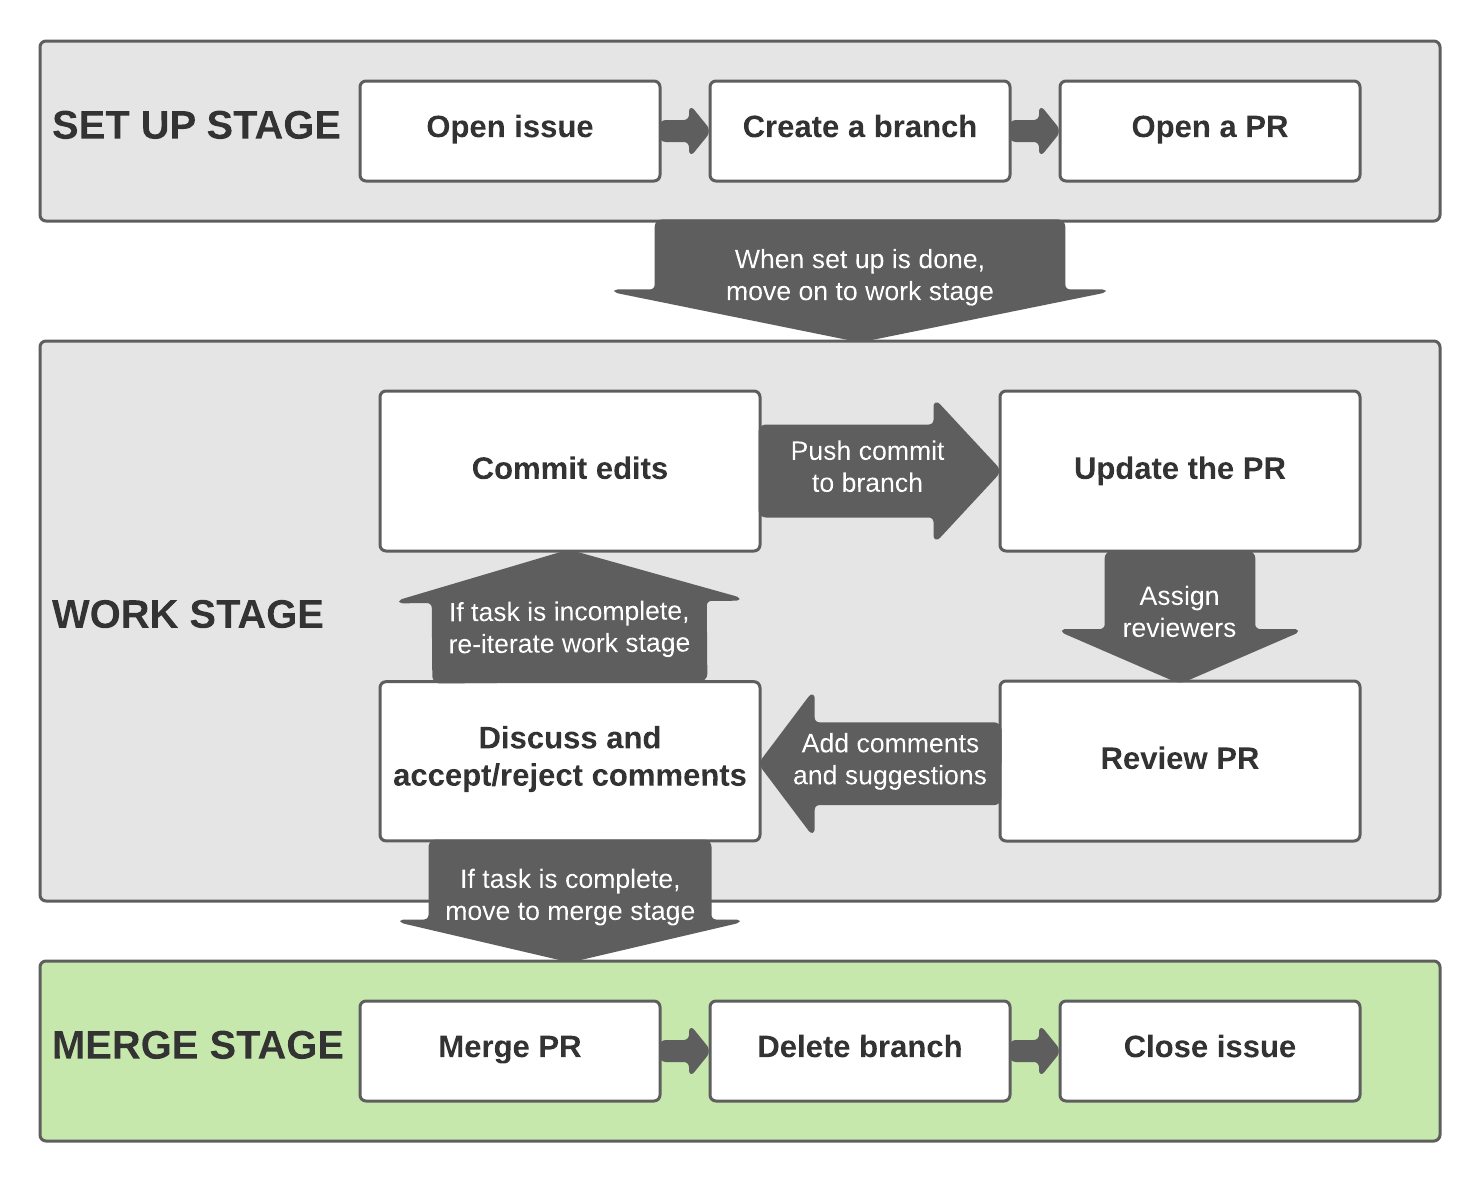
\includegraphics[width=\textwidth]{./img/branch-pr-merge-cycle-S3.png}
		\end{figure}

	\end{columns}
\end{frame}


\begin{frame}
	\frametitle{Merge the PR}
	\begin{columns}[c]

		\column{.35\textwidth} % Left column and width
		\begin{itemize}
			\setlength\itemsep{.5em}
			\item Make sure that the PR is well documented
			- this is where future team members will read
			how something was done and why
			\item Then you can merge your well-reviewed and well-documented code
			\item \textbf{Test run your code after merging it!}

		\end{itemize}

		\column{.65\textwidth} % Right column and width
		\vspace{-.75cm}
		\begin{figure}
			\centering
			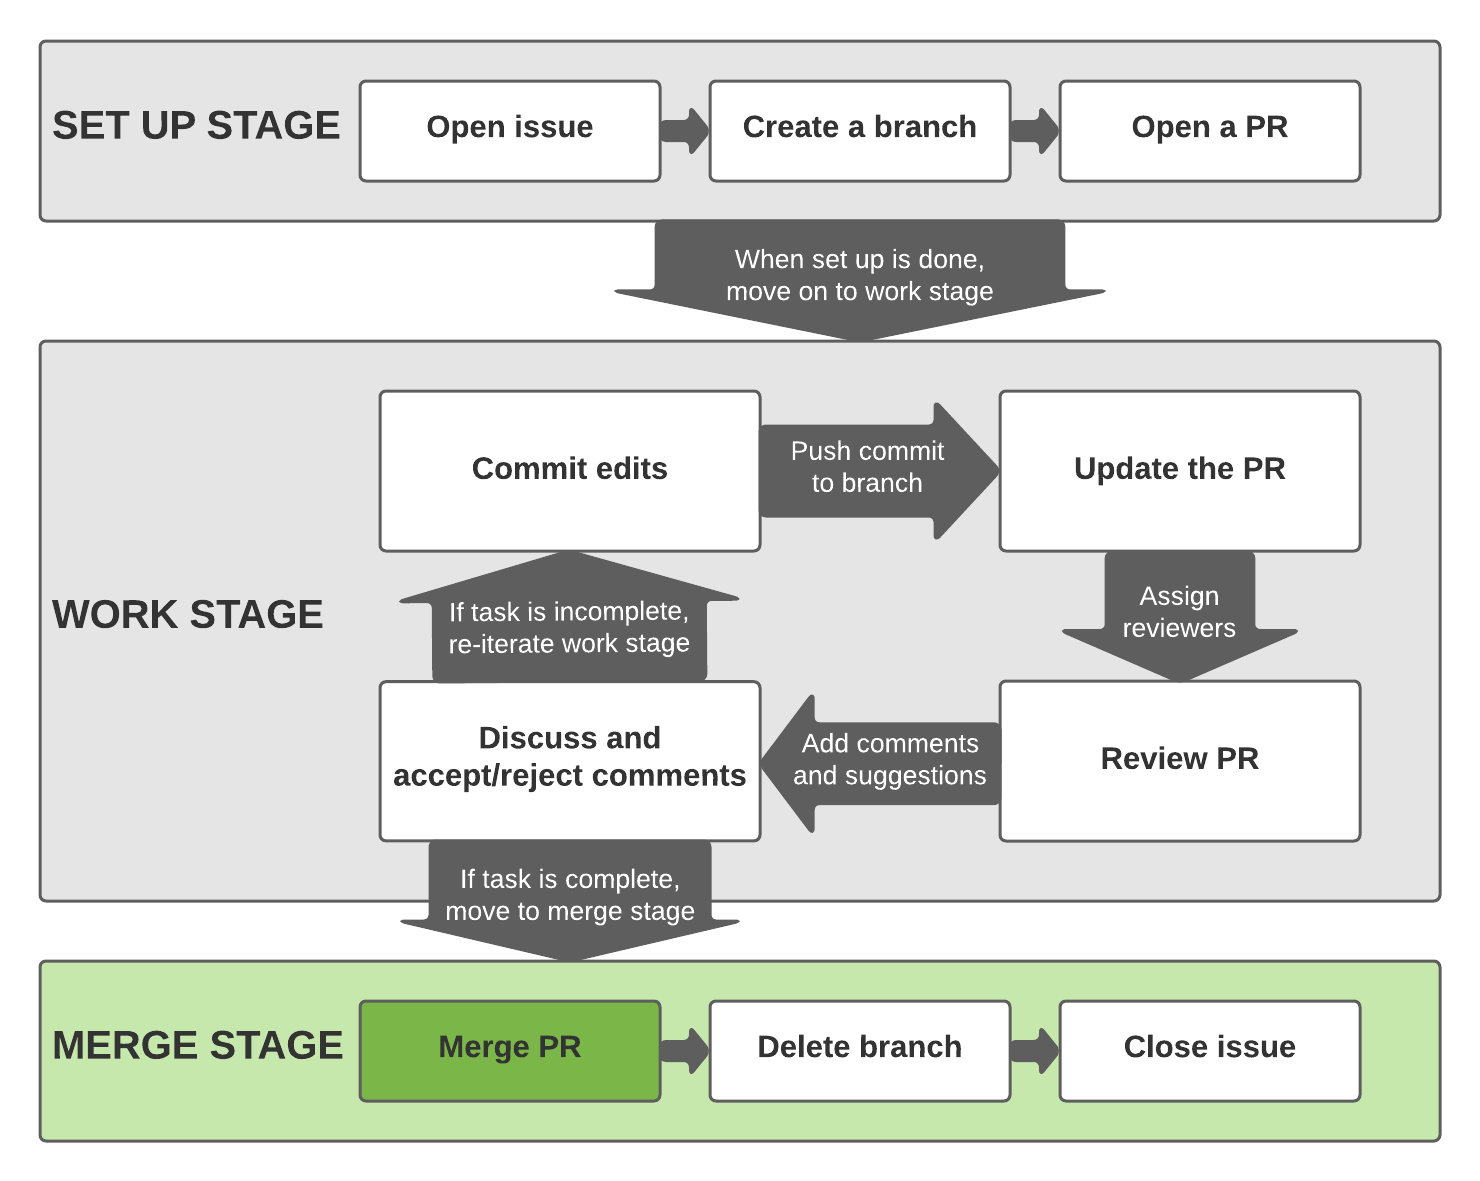
\includegraphics[width=\textwidth]{./img/branch-pr-merge-cycle-S3-1.png}
		\end{figure}

	\end{columns}
\end{frame}

\begin{frame}
	\frametitle{Delete the branch}
	\begin{columns}[c]

		\column{.35\textwidth} % Left column and width
		\begin{itemize}
			\setlength\itemsep{1em}
			\item Always delete branches after they are merged
			\item If you want to keep working in a branch with the same name,
			then re-create that branch
			\item Otherwise you risk working on an outdated version of the repo
		\end{itemize}

		\column{.65\textwidth} % Right column and width
		\vspace{-.75cm}
		\begin{figure}
			\centering
			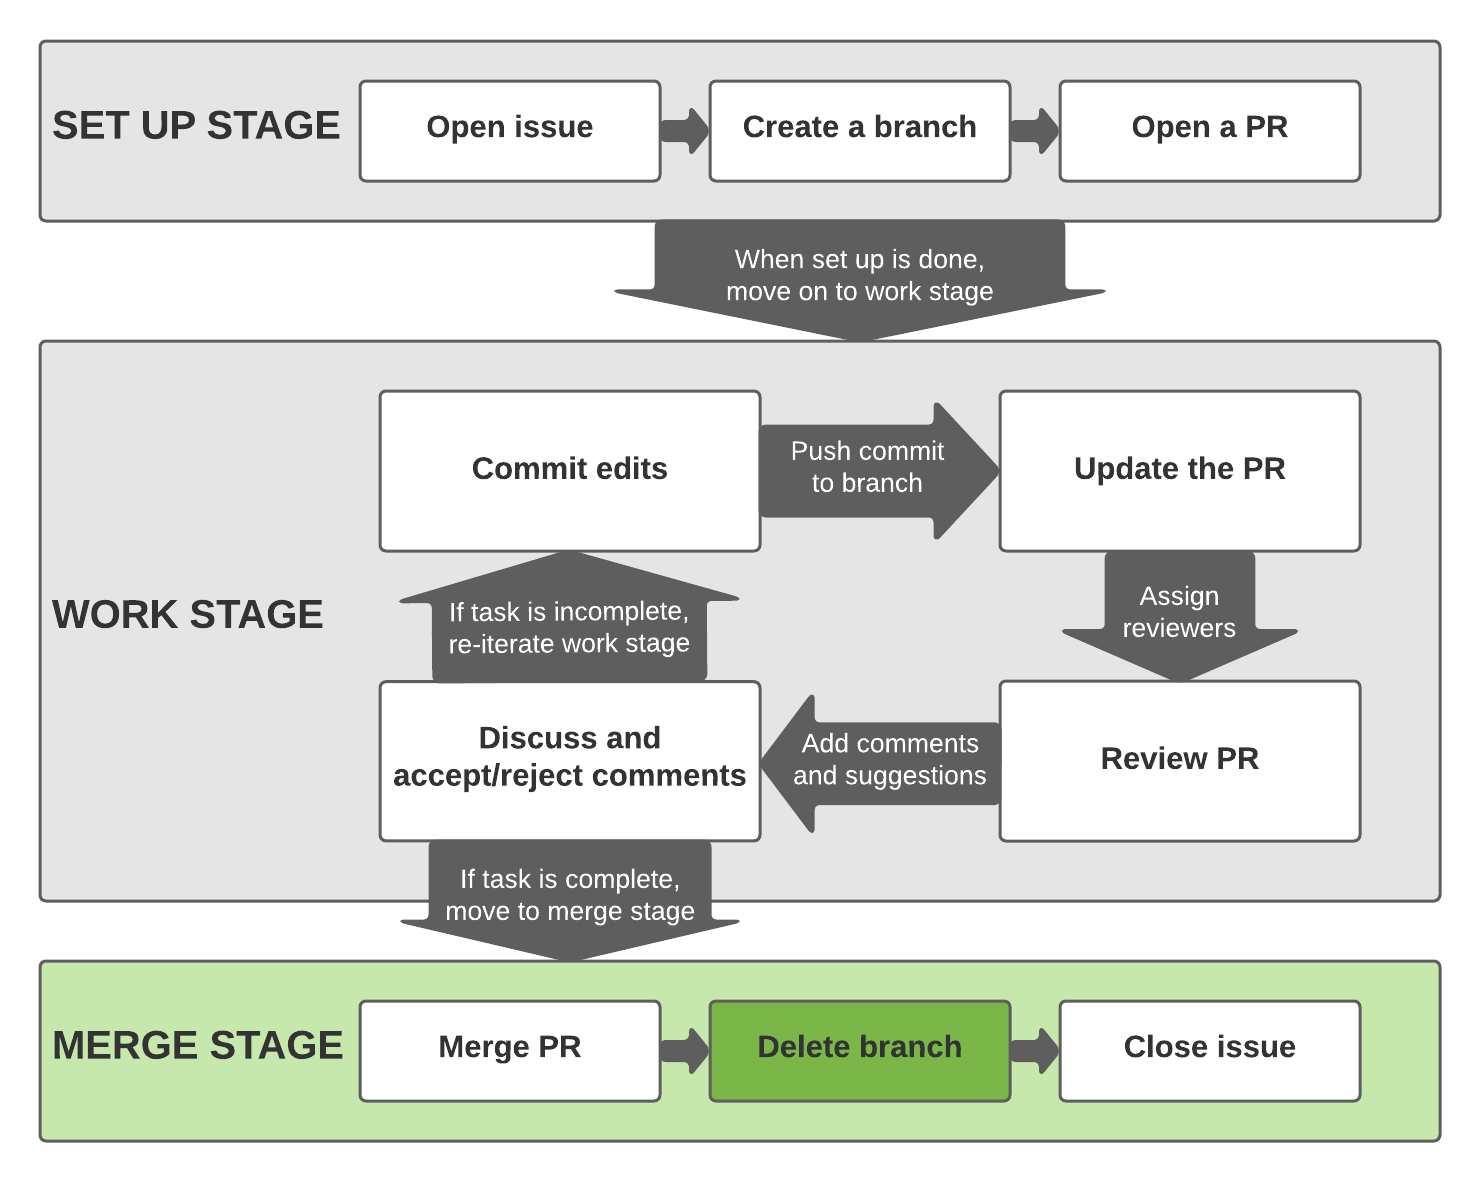
\includegraphics[width=\textwidth]{./img/branch-pr-merge-cycle-S3-2.png}
		\end{figure}

	\end{columns}
\end{frame}

\begin{frame}
	\frametitle{Close issue}
	\begin{columns}[c]

		\column{.35\textwidth} % Left column and width
		If you created an issue for this task:
		\begin{itemize}
			\setlength\itemsep{.5em}
			\item Make sure that the PR number is referenced in the issue.
			\item For example: \textit{``Issue resolved in PR \#12''}
			\item Then close the issue
		\end{itemize}

		\column{.65\textwidth} % Right column and width
		\vspace{-.75cm}
		\begin{figure}
			\centering
			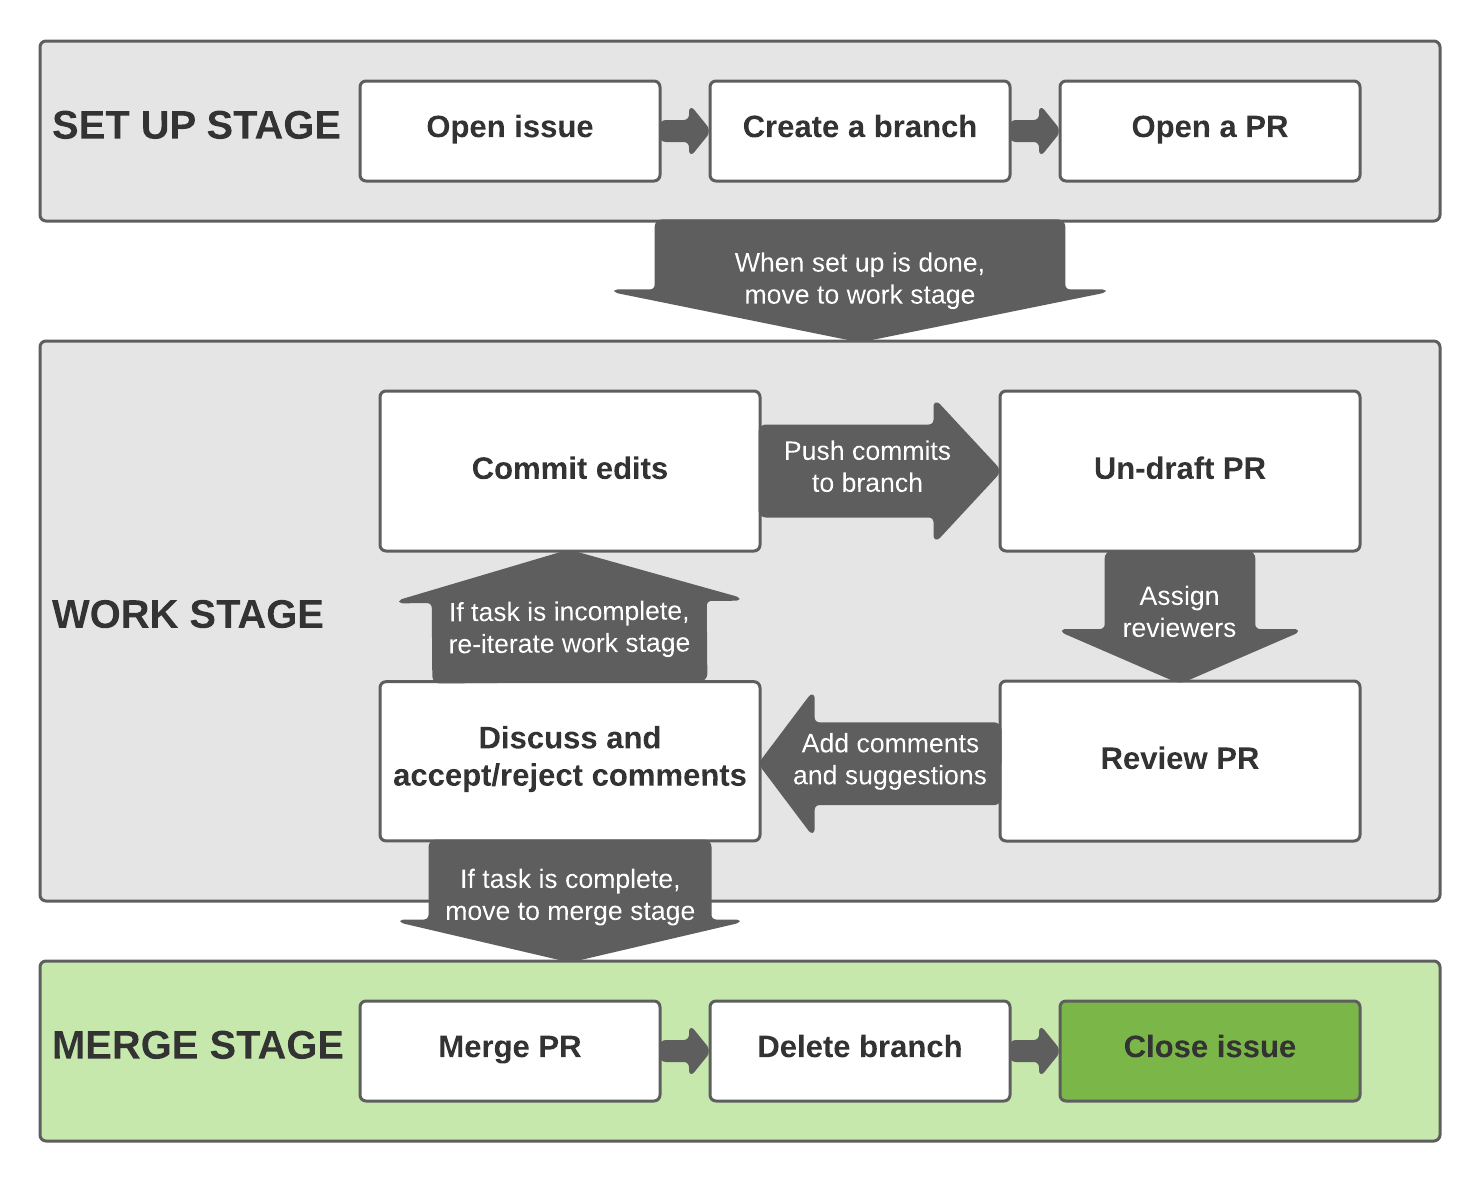
\includegraphics[width=\textwidth]{./img/branch-pr-merge-cycle-S3-3.png}
		\end{figure}

	\end{columns}
\end{frame}



\section{Part 2: \newline Gitflow - How to fit the ``branch-PR-merge'' cycle into your workflow}

\begin{frame}
	\frametitle{The network graph}

	\vspace{-.5cm}
	\begin{minipage}[t][5cm][t]{\textwidth}
		\begin{figure}
			\centering
			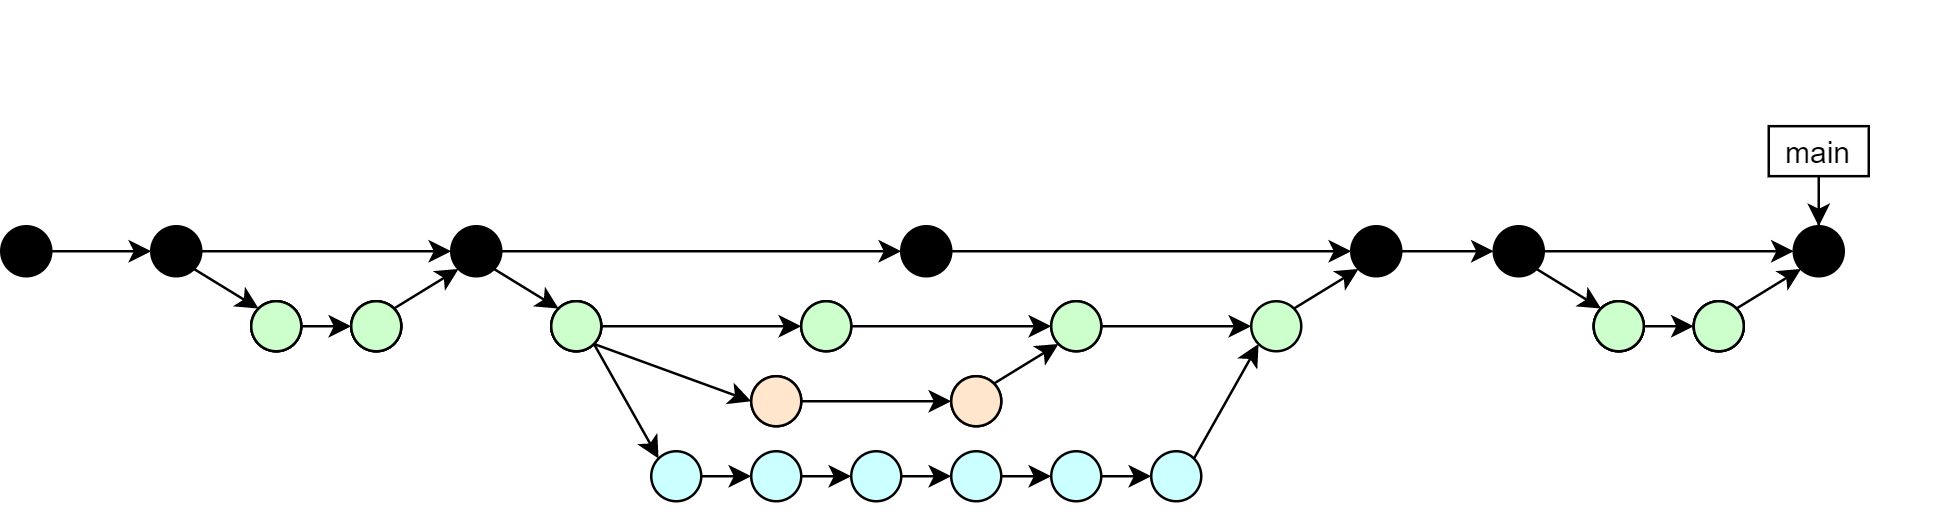
\includegraphics[width=\textwidth]{./img/dime-gitflow-network.png}
		\end{figure}
	\end{minipage}

	\vspace{-.5cm}
	\begin{minipage}[t][5cm][t]{\textwidth}
		\begin{itemize}
			\setlength\itemsep{.5em}
			\item A typical git network graph - each dot is a commit
			\item Several branches have been opened and merged,
			but currently only the \textit{main} branch is open
		\end{itemize}
	\end{minipage}

\end{frame}

\begin{frame}
	\frametitle{Gitflow}
	\begin{columns}[c]

		\column{.65\textwidth} % Left column and width
		\begin{itemize}
			\setlength\itemsep{.5em}
			\item Gitflow is not a software,
			it is an idea or a philosophy of how to organize work in git
			\item It is developed for computer science and
			you will find a lot of resources for it online
			\item We will present a simplified version adapted for research
			\item The \textbf{main branch} (formerly master branch)
			- should never be worked in directly
			\item \textbf{Feature branches} - this is where you do all your work
		\end{itemize}

		\column{.35\textwidth} % Right column and width
		\vspace{-.75cm}
		\begin{figure}
			\centering
			
\includegraphics[width=.75\textwidth]{./img/organization.png}
		\end{figure}
	\end{columns}
\end{frame}



\begin{frame}
	\frametitle{Simple branch-PR-merge cycle}

	\huge\centering \textbf{Simple branch-PR-merge cycle}

\end{frame}


\begin{frame}
	\frametitle{Start a branch-PR-merge cycle}

	\vspace{-.5cm}
	\begin{minipage}[t][5cm][t]{\textwidth}
		\begin{figure}
			\centering
			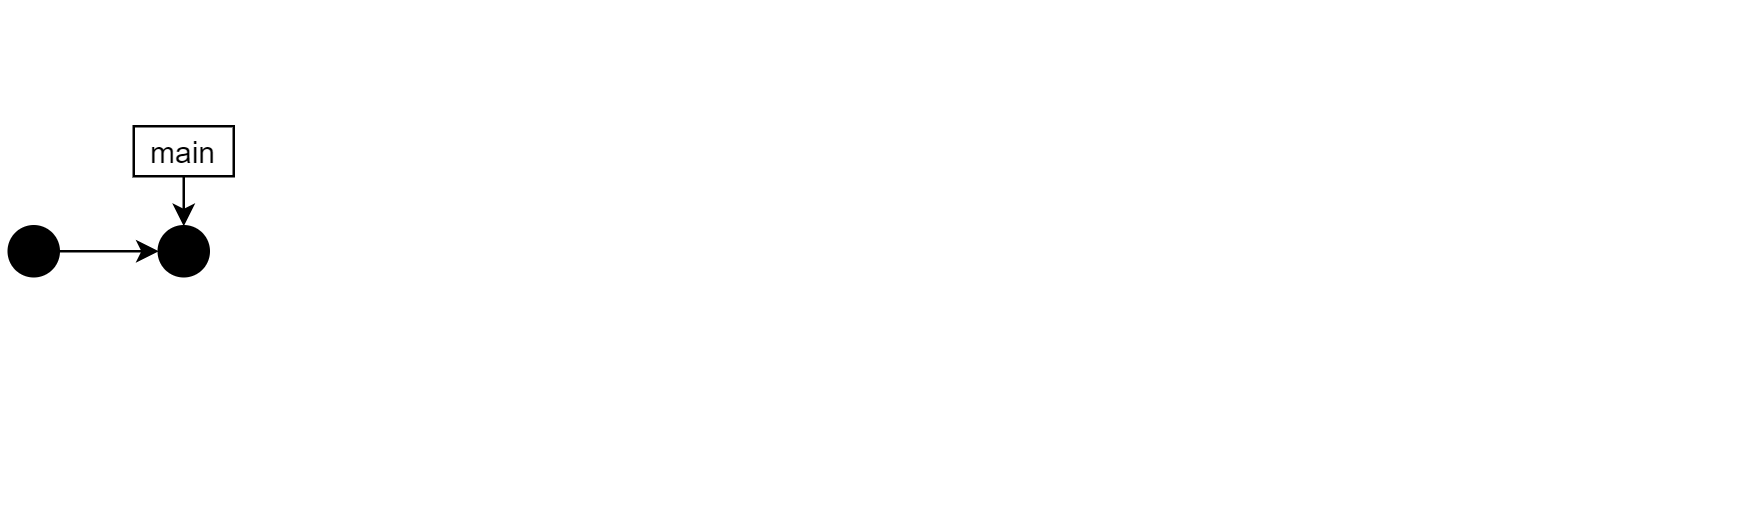
\includegraphics[width=\textwidth]{./img/dime-gitflow-network-0.png}
		\end{figure}
	\end{minipage}

	\vspace{-.5cm}
	\begin{minipage}[t][5cm][t]{\textwidth}
		\begin{itemize}
			\setlength\itemsep{.5em}
			\item This can either be the beginning of a repo
			or at a point where all previous branches were merged
			to the main branch
			\item Let's say your next task is to set up folders
			- apply the \textit{branch-PR-merge} cycle
		\end{itemize}
	\end{minipage}

\end{frame}


\begin{frame}
	\frametitle{Set up stage - 1}

	\vspace{-.5cm}
	\begin{minipage}[t][5cm][t]{\textwidth}
		\begin{figure}
			\centering
			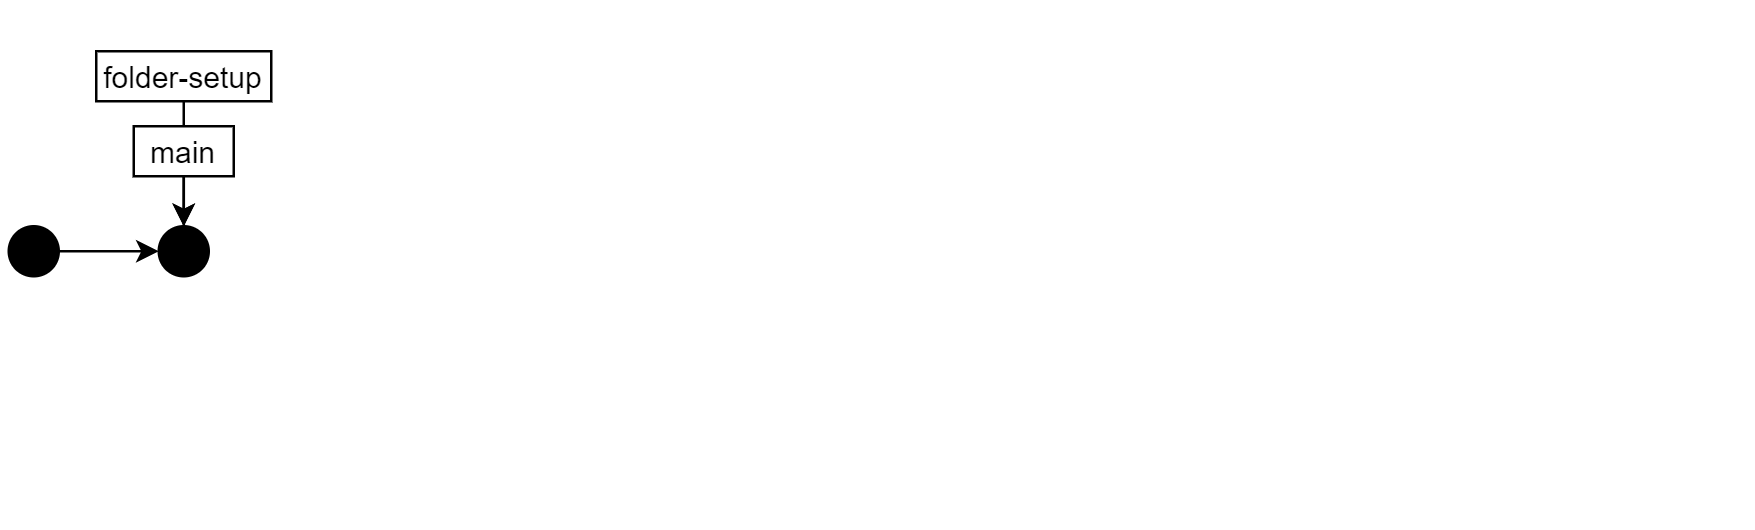
\includegraphics[width=\textwidth]{./img/dime-gitflow-network-1-0.png}
		\end{figure}
	\end{minipage}

	\vspace{-.5cm}
	\begin{minipage}[t][5cm][t]{\textwidth}
		\begin{itemize}
			\setlength\itemsep{.5em}
			\item Create a new \textit{feature} branch at the point
			where you want the the \textit{branch-PR-merge} cycle
			to start from
			\item Two branches pointing to the same commit
			are identical by definition
		\end{itemize}
	\end{minipage}

\end{frame}


\begin{frame}
	\frametitle{Set up stage - 2}

	\vspace{-.5cm}
	\begin{minipage}[t][5cm][t]{\textwidth}
		\begin{figure}
			\centering
			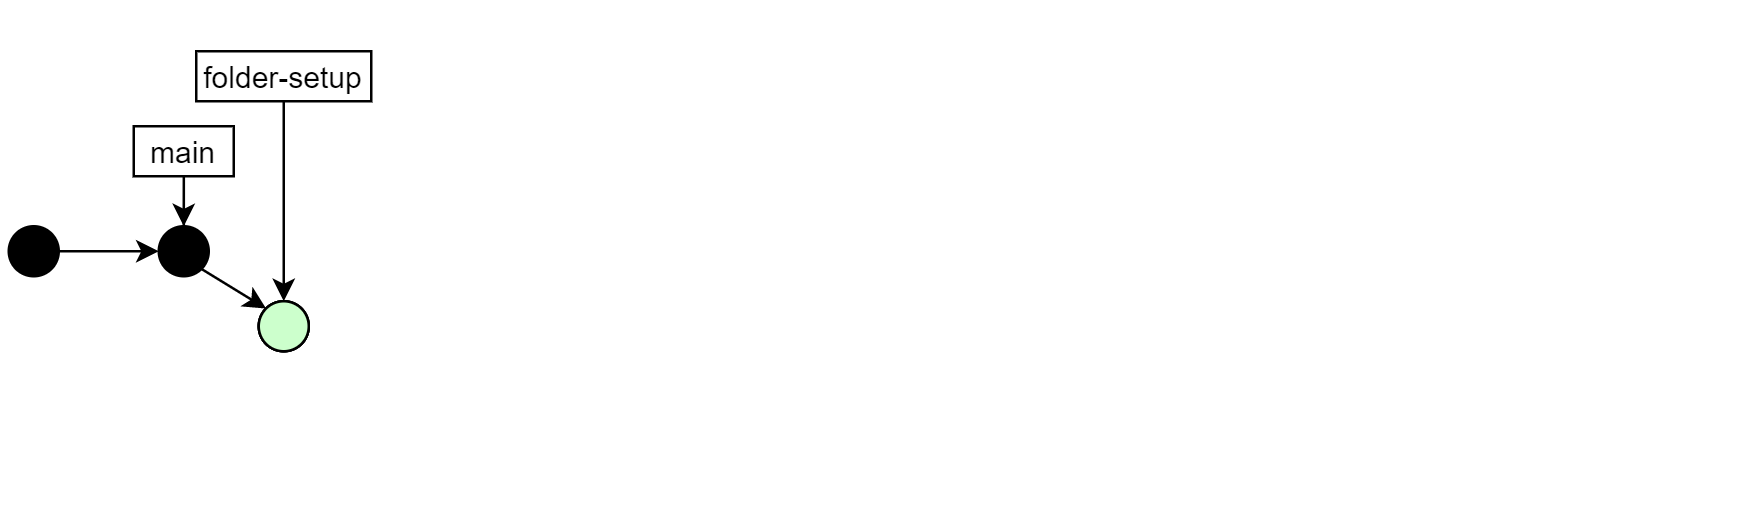
\includegraphics[width=\textwidth]{./img/dime-gitflow-network-1-1.png}
		\end{figure}
	\end{minipage}

	\vspace{-.5cm}
	\begin{minipage}[t][5cm][t]{\textwidth}
		\begin{itemize}
			\setlength\itemsep{.5em}
			\item Create a new short README or
			quickly edit an existing and commit -
			(or make a quick commit for the task) -
			at least one commit is needed for this work flow
			\item Open up a draft PR so there is a good place
			for your team to follow your work
		\end{itemize}
	\end{minipage}

\end{frame}

\begin{frame}
	\frametitle{Work stage}

	\vspace{-.5cm}
	\begin{minipage}[t][5cm][t]{\textwidth}
		\begin{figure}
			\centering
			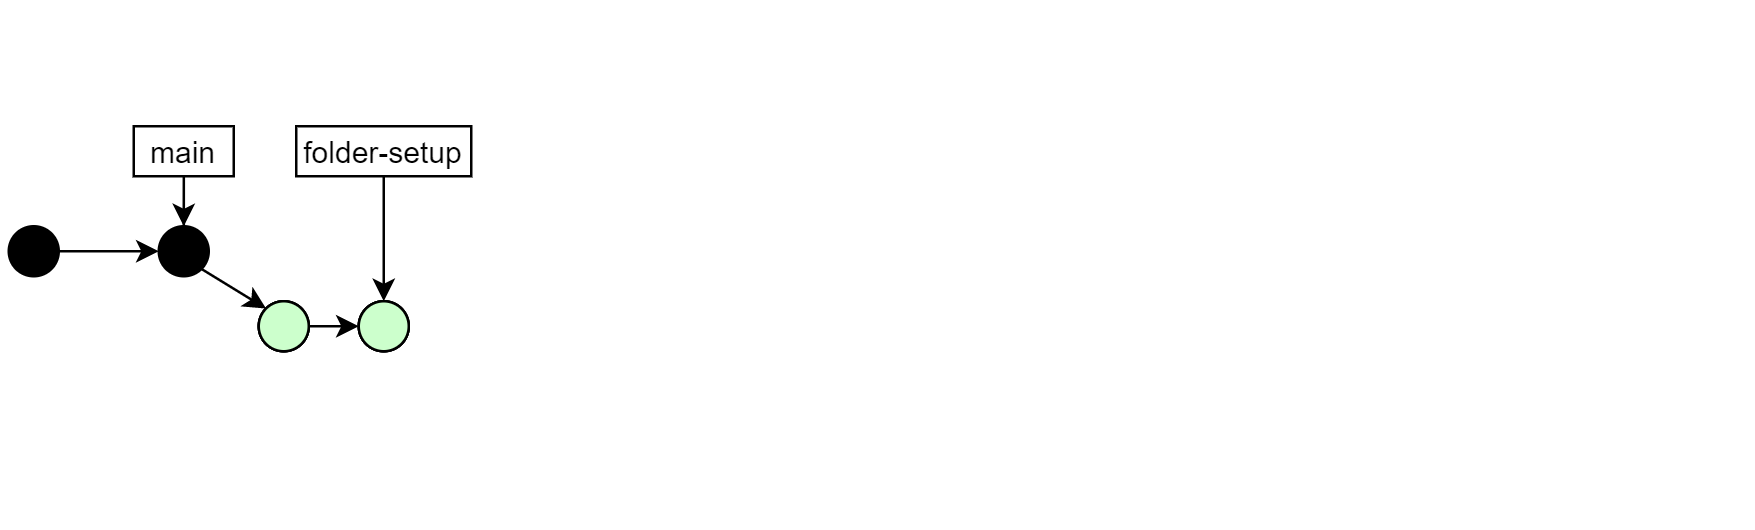
\includegraphics[width=\textwidth]{./img/dime-gitflow-network-1-2.png}
		\end{figure}
	\end{minipage}

	\vspace{-.5cm}
	\begin{minipage}[t][5cm][t]{\textwidth}
		\begin{itemize}
			\setlength\itemsep{.5em}
			\item Complete the task using one or many commits
			- this example only requires one more commit
			\item Assign someone to review the PR
			- iterate until you are all satisfied
		\end{itemize}
	\end{minipage}

\end{frame}

\begin{frame}
	\frametitle{Merge stage}

	\vspace{-.5cm}
	\begin{minipage}[t][5cm][t]{\textwidth}
		\begin{figure}
			\centering
			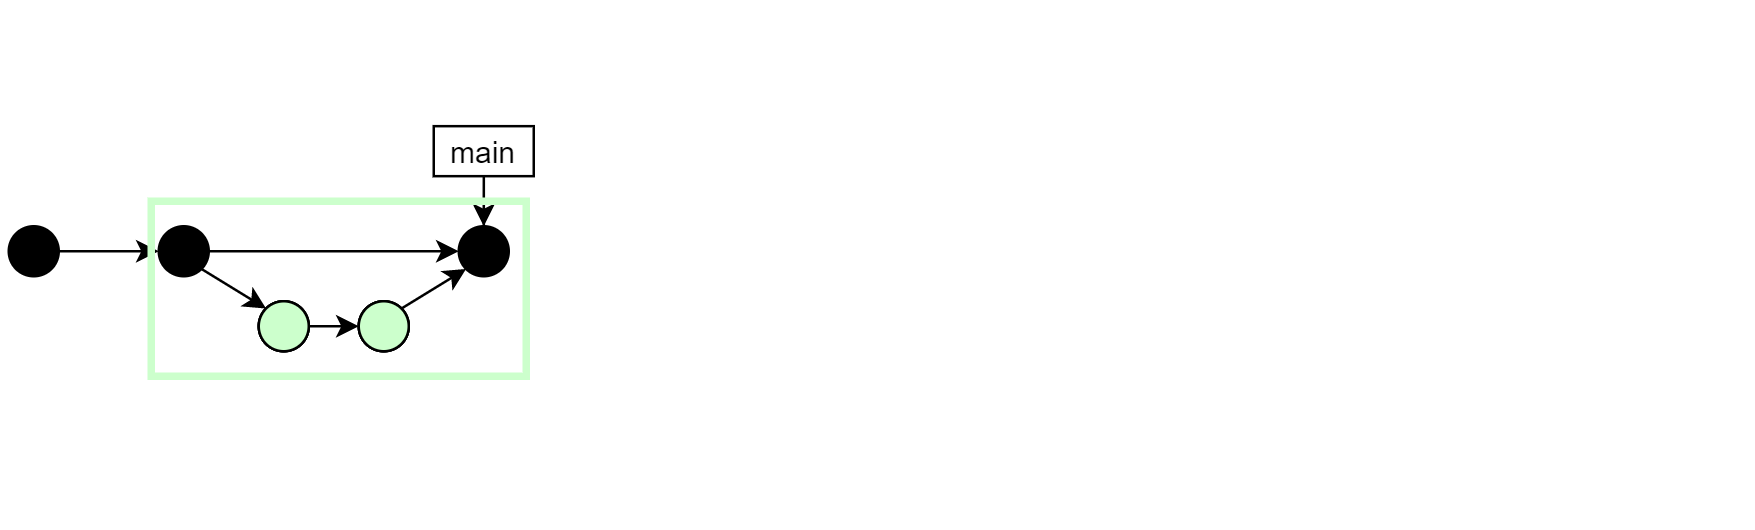
\includegraphics[width=\textwidth]{./img/dime-gitflow-network-1-3.png}
		\end{figure}
	\end{minipage}

	\vspace{-.5cm}
	\begin{minipage}[t][5cm][t]{\textwidth}
		\begin{itemize}
			\setlength\itemsep{.5em}
			\item Merge the PR
			\item Delete the \textit{feature} branch
			\item The green box represents
			a full \textit{branch-PR-merge} cycle in the network graph
		\end{itemize}
	\end{minipage}

\end{frame}

\begin{frame}
	\frametitle{Nested branch-PR-merge cycles}

	\huge\centering \textbf{Nested branch-PR-merge cycles}

\end{frame}

\begin{frame}
	\frametitle{Nested branch-PR-merge cycles}
	\begin{columns}[c]

		\column{.65\textwidth} % Left column and width
		\begin{itemize}
			\setlength\itemsep{.5em}
			\item Many high-level tasks are not simple
			- multiple team members working over multiple months
			\item Cleaning the baseline data,
			for example, is one big task composed of many smaller tasks
			\item Solve this by using nested \textit{branch-PR-merge} cycles
			\item \textbf{Develop branch}
			- a branch that is a high-level task that
			will have several \textit{feature} branches
		\end{itemize}

		\column{.35\textwidth} % Right column and width

		\begin{figure}
			\centering
			
\includegraphics[width=.65\textwidth]{./img/team-challenge.png}
		\end{figure}
	\end{columns}
\end{frame}

\begin{frame}
	\frametitle{Create a develop branch}

	\vspace{-.5cm}
	\begin{minipage}[t][5cm][t]{\textwidth}
		\begin{figure}
			\centering
			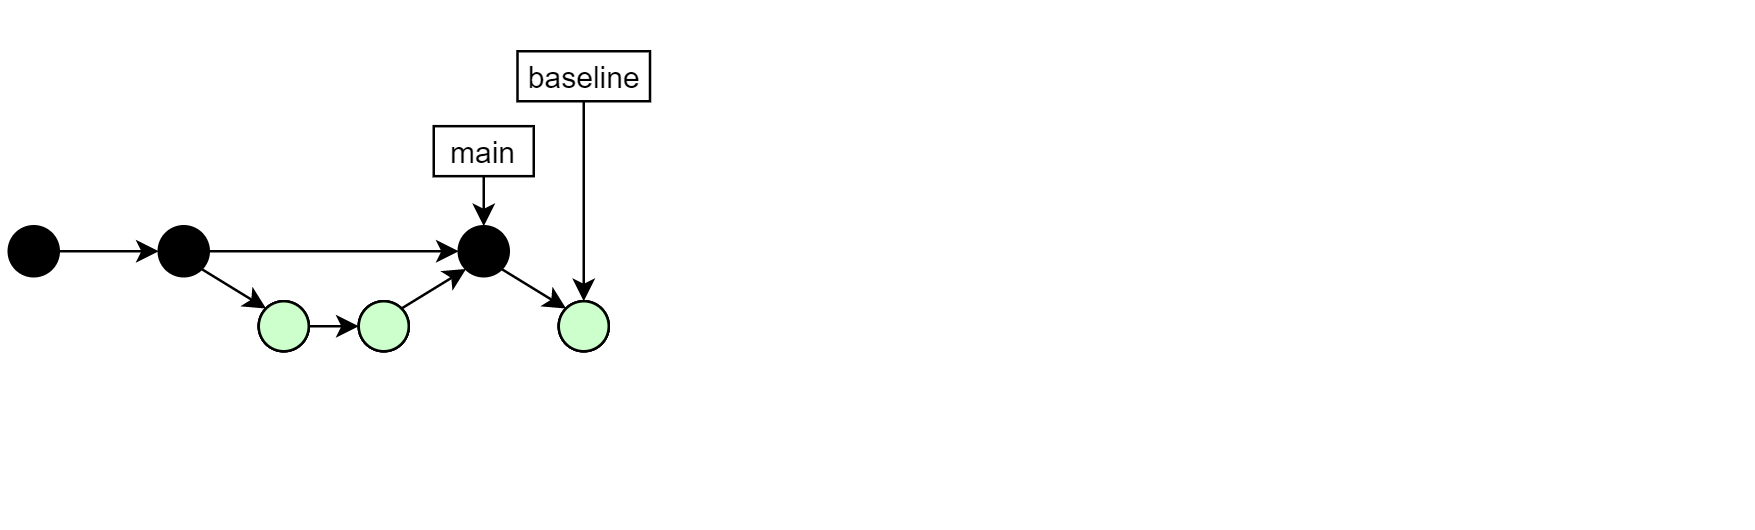
\includegraphics[width=\textwidth]{./img/dime-gitflow-network-2-1.png}
		\end{figure}
	\end{minipage}

	\vspace{-.5cm}
	\begin{minipage}[t][5cm][t]{\textwidth}
		\begin{itemize}
			\setlength\itemsep{.5em}
			\item Create a \textit{develop} branch
			- name it after the high-level task
			- complete set up stage
			\item \textit{Develop} branches often do not have a Github issue
			- but the \textit{feature} branches off of it
			should often have an corresponding GitHub issue
			\item Include \textit{develop} branch name as prefix
			to all \textit{feature} branches off it
		\end{itemize}
	\end{minipage}
\end{frame}

\begin{frame}
	\frametitle{Create feature branches of the develop branch}

	\vspace{-.5cm}
	\begin{minipage}[t][5cm][t]{\textwidth}
		\begin{figure}
			\centering
			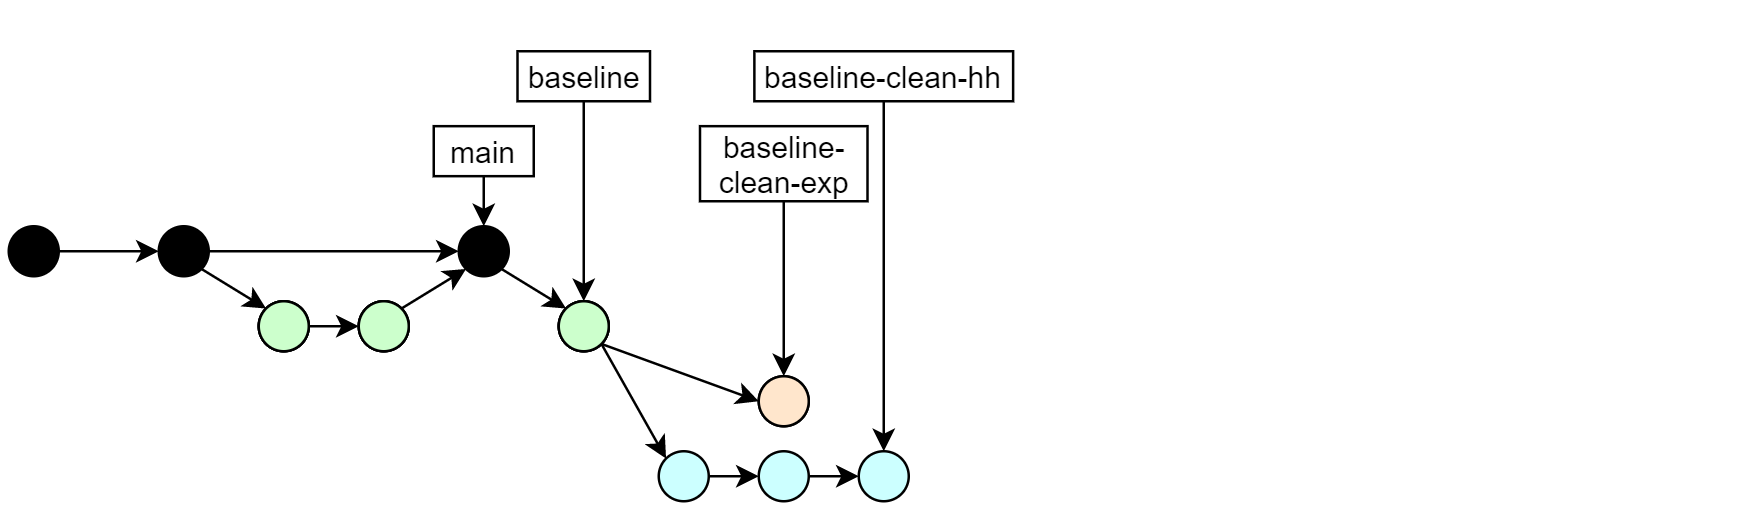
\includegraphics[width=\textwidth]{./img/dime-gitflow-network-2-2.png}
		\end{figure}
	\end{minipage}

	\vspace{-.5cm}
	\begin{minipage}[t][5cm][t]{\textwidth}
		\begin{itemize}
			\setlength\itemsep{.5em}
			\item Create as many \textit{feature} branches off
			the \textit{develop} branch as you need
			\item Split up the high-level task in as many smaller tasks as needed
			- try to split up tasks until each is small enough
			for one person to complete in a week or two
			\item Create new \textit{feature} branches off
			the \textit{develop} branch even after it progresses
		\end{itemize}
	\end{minipage}
\end{frame}

\begin{frame}
	\frametitle{Work in the branches}

	\vspace{-.5cm}
	\begin{minipage}[t][5cm][t]{\textwidth}
		\begin{figure}
			\centering
			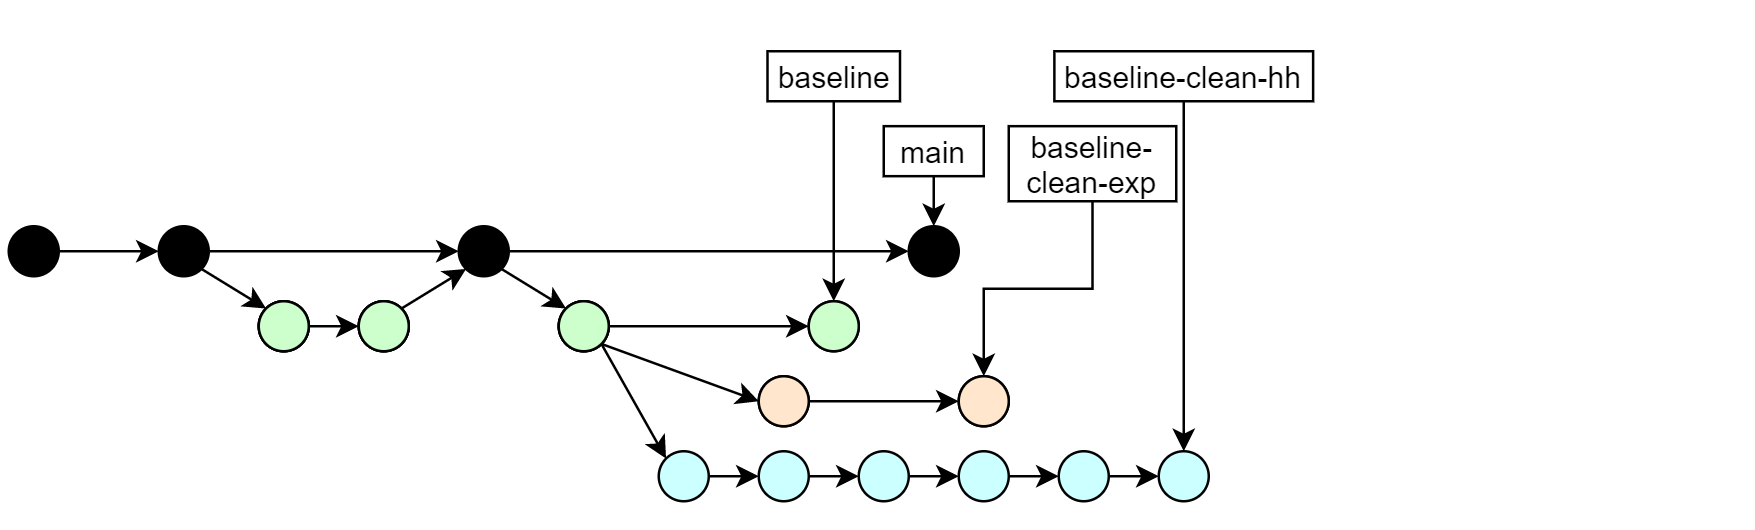
\includegraphics[width=\textwidth]{./img/dime-gitflow-network-2-3.png}
		\end{figure}
	\end{minipage}

	\vspace{-.5cm}
	\begin{minipage}[t][5cm][t]{\textwidth}
		\begin{itemize}
			\setlength\itemsep{.5em}
			\item Keep working on the \textit{feature} branches until
			they are done
			\item When a task is complete: assign a reviewer
			- comment/suggest - accept/reject/discuss
		\end{itemize}
	\end{minipage}
\end{frame}

\begin{frame}
	\frametitle{Merge a feature branch}

	\vspace{-.5cm}
	\begin{minipage}[t][5cm][t]{\textwidth}
		\begin{figure}
			\centering
			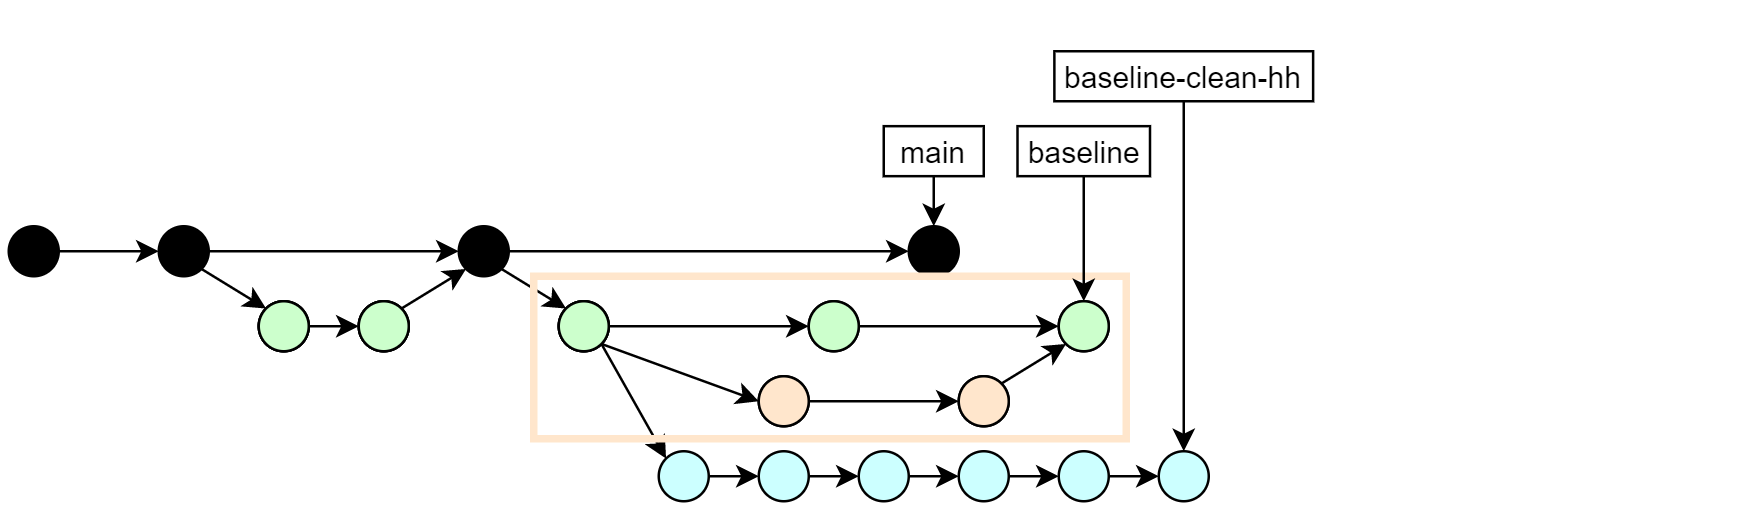
\includegraphics[width=\textwidth]{./img/dime-gitflow-network-2-4.png}
		\end{figure}
	\end{minipage}

	\vspace{-.5cm}
	\begin{minipage}[t][5cm][t]{\textwidth}
		\begin{itemize}
			\setlength\itemsep{.5em}
			\item The branch \texttt{baseline-clean-exp} was
			approved in the last step in the work stage and
			was merged and deleted in the merge stage
			\item The orange box is one \textit{branch-PR-merge} cycle
		\end{itemize}
	\end{minipage}
\end{frame}

\begin{frame}
	\frametitle{Merge a feature branch}

	\vspace{-.5cm}
	\begin{minipage}[t][5cm][t]{\textwidth}
		\begin{figure}
			\centering
			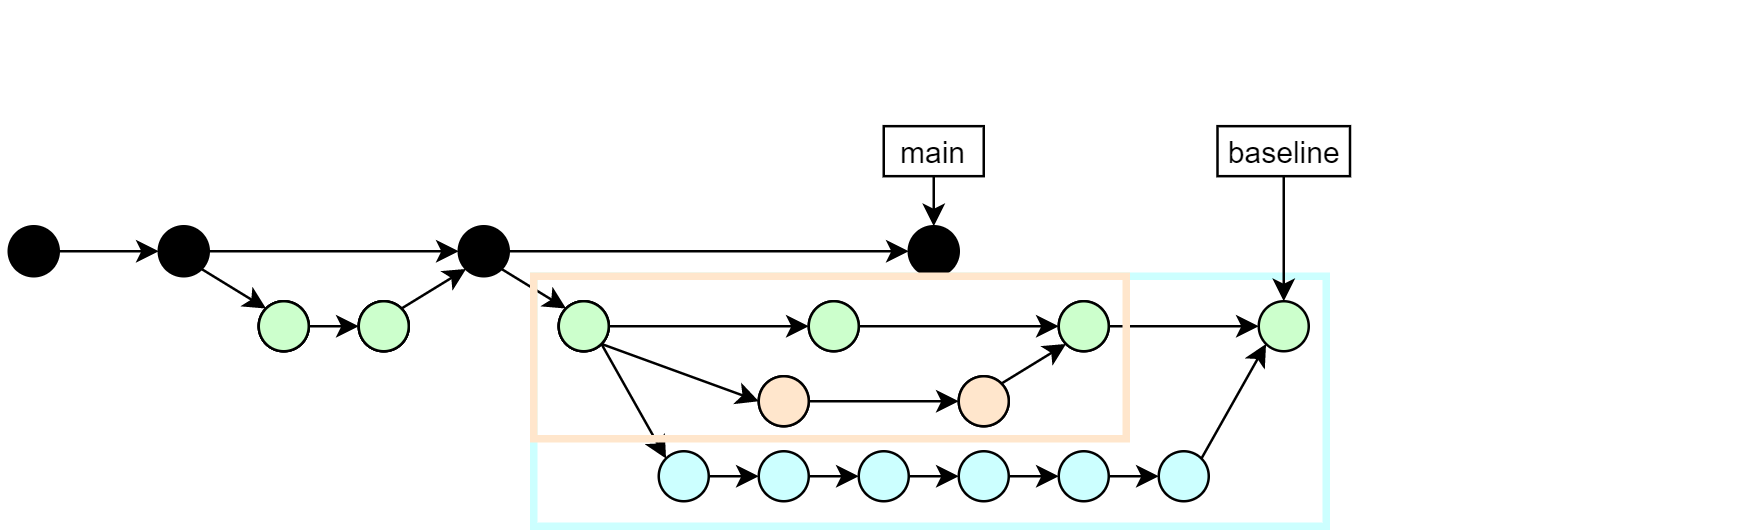
\includegraphics[width=\textwidth]{./img/dime-gitflow-network-2-5.png}
		\end{figure}
	\end{minipage}

	\vspace{-.5cm}
	\begin{minipage}[t][5cm][t]{\textwidth}
		\begin{itemize}
			\setlength\itemsep{.5em}
			\item The branch \texttt{baseline-clean-hh} was then
			also approved in the last step in the work stage and
			was merged and deleted in the merge stage
			\item The blue box is also a \textit{branch-PR-merge} cycle
		\end{itemize}
	\end{minipage}
\end{frame}

\begin{frame}
	\frametitle{Merge a develop branch}

	\vspace{-.5cm}
	\begin{minipage}[t][5cm][t]{\textwidth}
		\begin{figure}
			\centering
			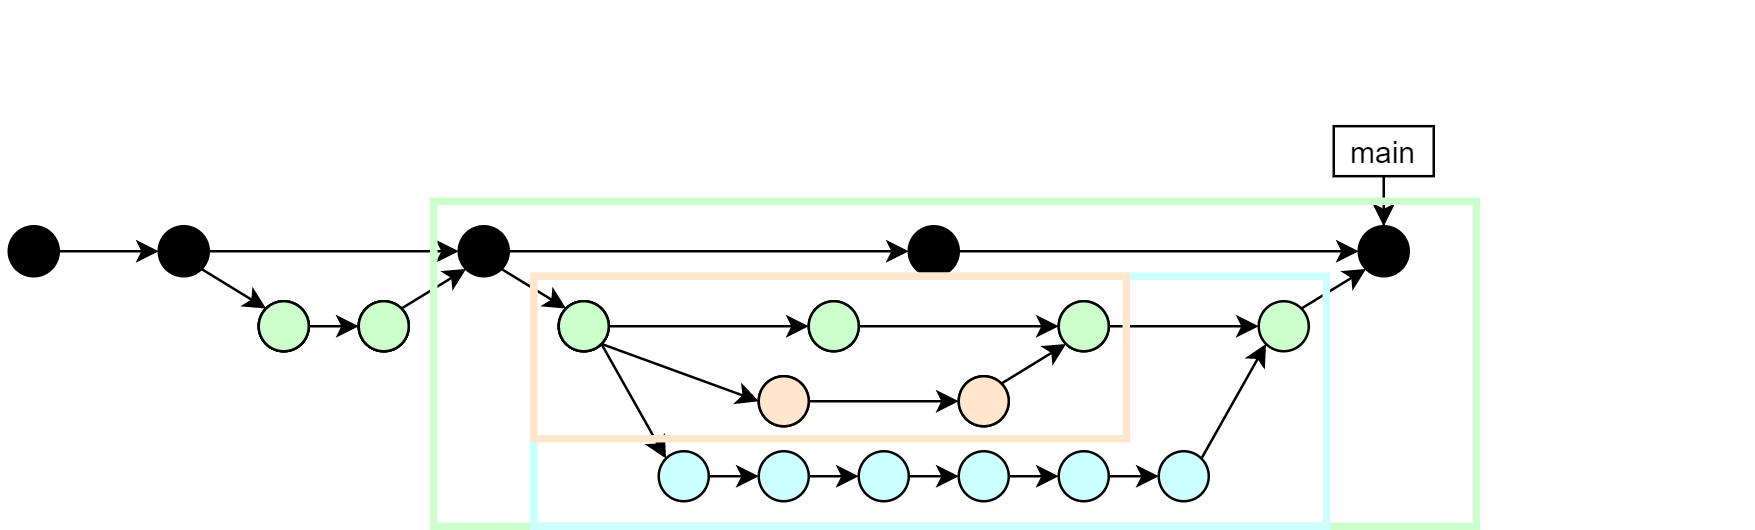
\includegraphics[width=\textwidth]{./img/dime-gitflow-network-2-6.png}
		\end{figure}
	\end{minipage}

	\vspace{-.5cm}
	\begin{minipage}[t][5cm][t]{\textwidth}
		\begin{itemize}
			\setlength\itemsep{.5em}
			\item Then the branch \texttt{baseline} is ready for a review
			- assign a reviewer - comment/suggest - accept/reject/discuss
			\item The green box is also a \textit{branch-PR-merge} cycle
			\item This network graph shows
			a nested \textit{branch-PR-merge} cycle
		\end{itemize}
	\end{minipage}
\end{frame}


\begin{frame}
	\frametitle{Work directly in main/develop}

	\vspace{-.5cm}
	\begin{minipage}[t][5cm][t]{\textwidth}
		\begin{figure}
			\centering
			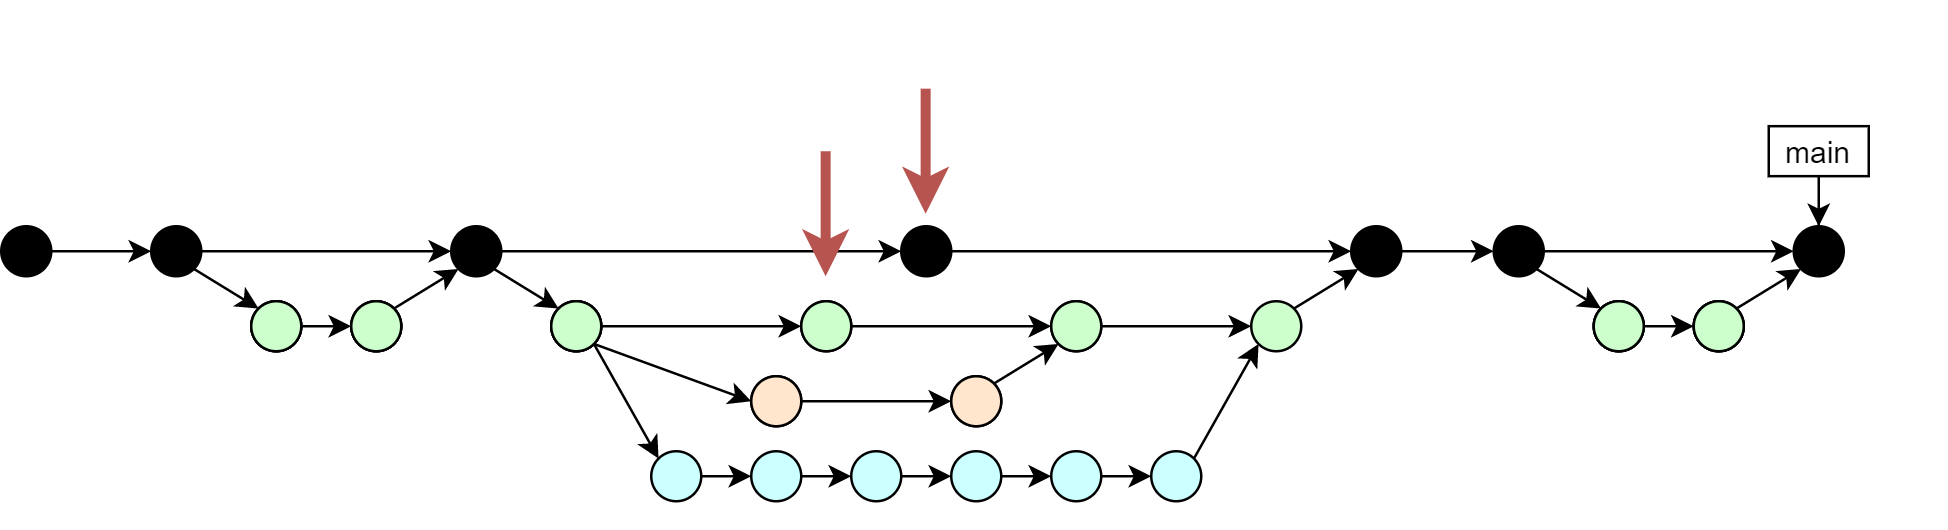
\includegraphics[width=\textwidth]{./img/dime-gitflow-network-workdirectly.png}
		\end{figure}
	\end{minipage}

	\vspace{-.5cm}
	\begin{minipage}[t][5cm][t]{\textwidth}
		\begin{itemize}
			\setlength\itemsep{.5em}
			\item <1->When could it be ok to work
			directly on a \textit{main}/\textit{develop} branch?
			- see red arrows
			\item <2->When updating documentation!
			\begin{itemize}
				\setlength\itemsep{.5em}
				\item <2->Documentation about the repo
				in the \textit{main} branch
				\item <2->Documentation about the high-level task
				in the \textit{develop} branch
			\end{itemize}
		\end{itemize}
	\end{minipage}
\end{frame}

\begin{frame}
	\frametitle{The network graph}

	\vspace{-.5cm}
	\begin{minipage}[t][5cm][t]{\textwidth}
		\begin{figure}
			\centering
			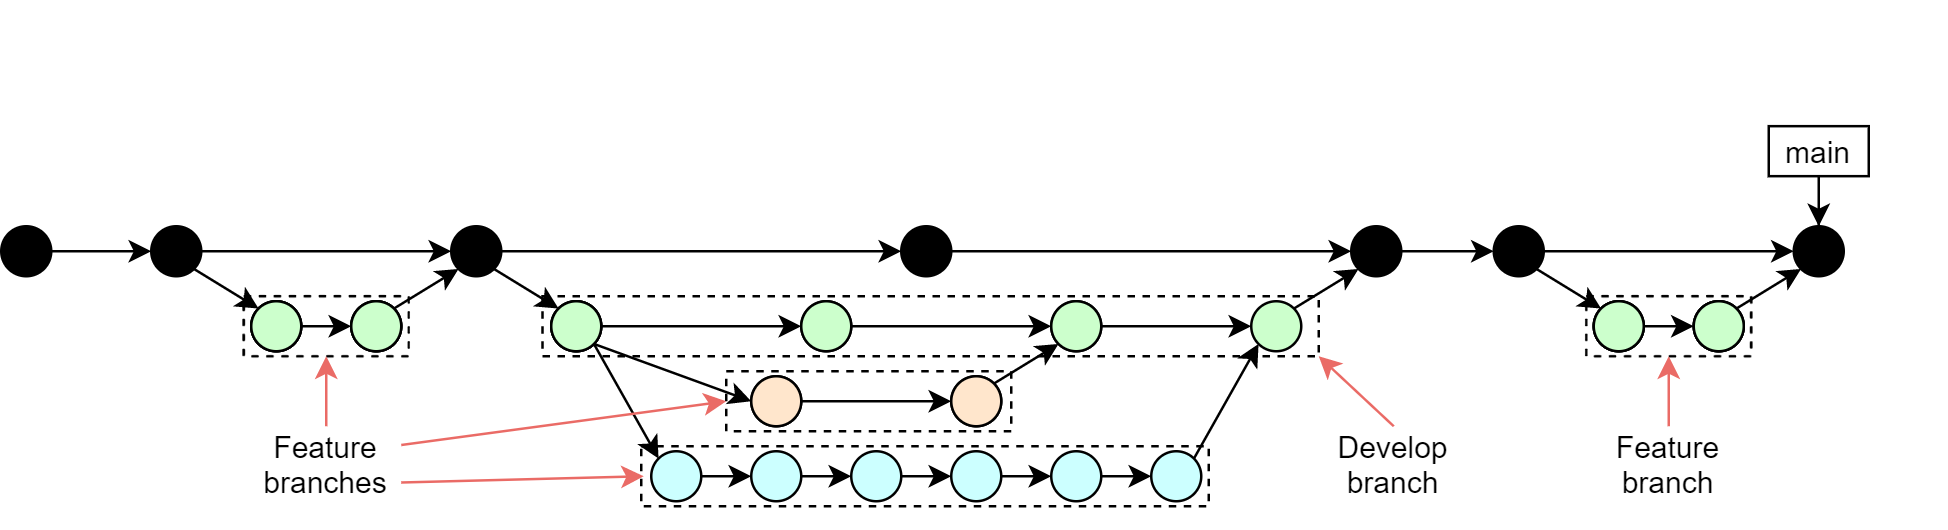
\includegraphics[width=\textwidth]{./img/dime-gitflow-network-names.png}
		\end{figure}
	\end{minipage}

	\vspace{-1cm}
	\begin{minipage}[t][5cm][t]{\textwidth}
		\begin{itemize}
			\setlength\itemsep{.4em}
			\item There is technically no difference between
			the Gitflow types of branches
			- the only difference is what workflow that is expected
			\begin{itemize}
				\setlength\itemsep{.5em}
				\item \textbf{Main branch}:
				The branch where all branches originates from
				\item \textbf{Develop branch}:
				Non-\textit{main} branch with \textit{feature} branches
				\item \textbf{Feature branch}:
				Branches of the \textit{main} branch or
				\textit{develop} branches with no other branches from it
			\end{itemize}
		\end{itemize}
	\end{minipage}
\end{frame}


\begin{frame}
	\frametitle{Nest cycles in the work stage}
	\begin{columns}[c]

		\column{.35\textwidth} % Left column and width
		\begin{itemize}
			\setlength\itemsep{1em}
			\item \textit{Branch-PR-merge} cycles should be nested
			in the work stage
			\item The \textit{develop} branch is paused
			in the \textit{Commit edits} step while
			feature \textit{branch-PR-merge} cycles are completed
			\item If needed, convert a \textit{feature} branch
			to a \textit{develop} branch here
		\end{itemize}

		\column{.65\textwidth} % Right column and width
		\vspace{-.75cm}
		\begin{figure}
			\centering
			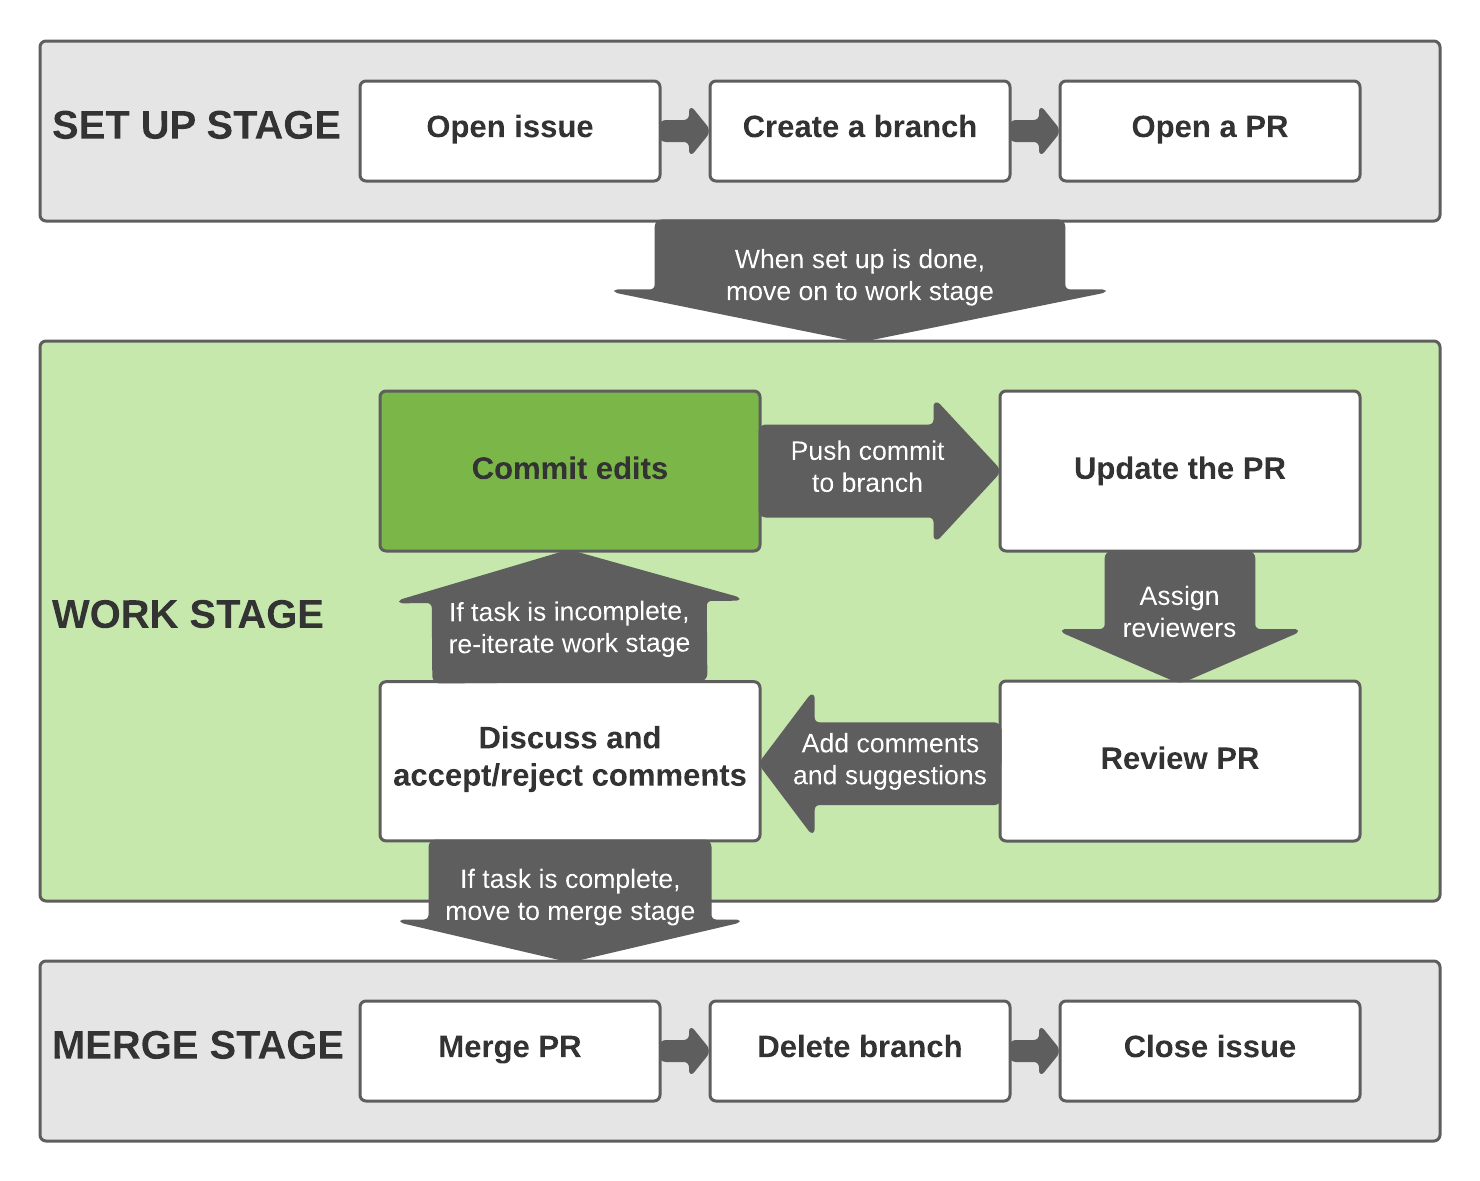
\includegraphics[width=\textwidth]{./img/branch-pr-merge-cycle-S2-1.png}
		\end{figure}
	\end{columns}
\end{frame}

\begin{frame}
	\frametitle{Thank you!}
	\huge\centering \textbf{Questions?}

	\vspace{1cm}
	\normalsize Slides can be found here: \url{https://osf.io/e54gy/}
\end{frame}

\begin{frame}{Useful links}
	\begin{itemize}
	  \item All DIME Analytics GitHub trainings: \trainingURL{https://osf.io/e54gy/}
	  \item Other DIME Analytics GitHub resources: \trainingURL{https://github.com/worldbank/dime-github-trainings}. For example:
		\begin{itemize}
			\item DIME Analytics GitHub Templates (for example .gitignore): \trainingURL{https://github.com/worldbank/dime-github-trainings/tree/master/GitHub-resources/DIME-GitHub-Templates}
			\item DIME Analytics GitHub Roles: \trainingURL{https://github.com/worldbank/dime-github-trainings/blob/master/GitHub-resources/DIME-GitHub-Roles/DIME-GitHub-roles.md}
		\end{itemize}
		\item Markdown cheat sheet (how to format text on GitHub.com):  \trainingURL{https://www.markdownguide.org/cheat-sheet/}
		\item DIME GitHub Account admin info and instructions: \trainingURL{https://github.com/dime-worldbank/dime-account-admin}
	\end{itemize}
\end{frame}


\input{../../Common-Resources/slides/GitHub-Commit-URL.tex}

\section{Appendix}

\begin{frame}{Create branch on GitHub.com}
\label{new-branch}

\begin{figure}
	\centering
	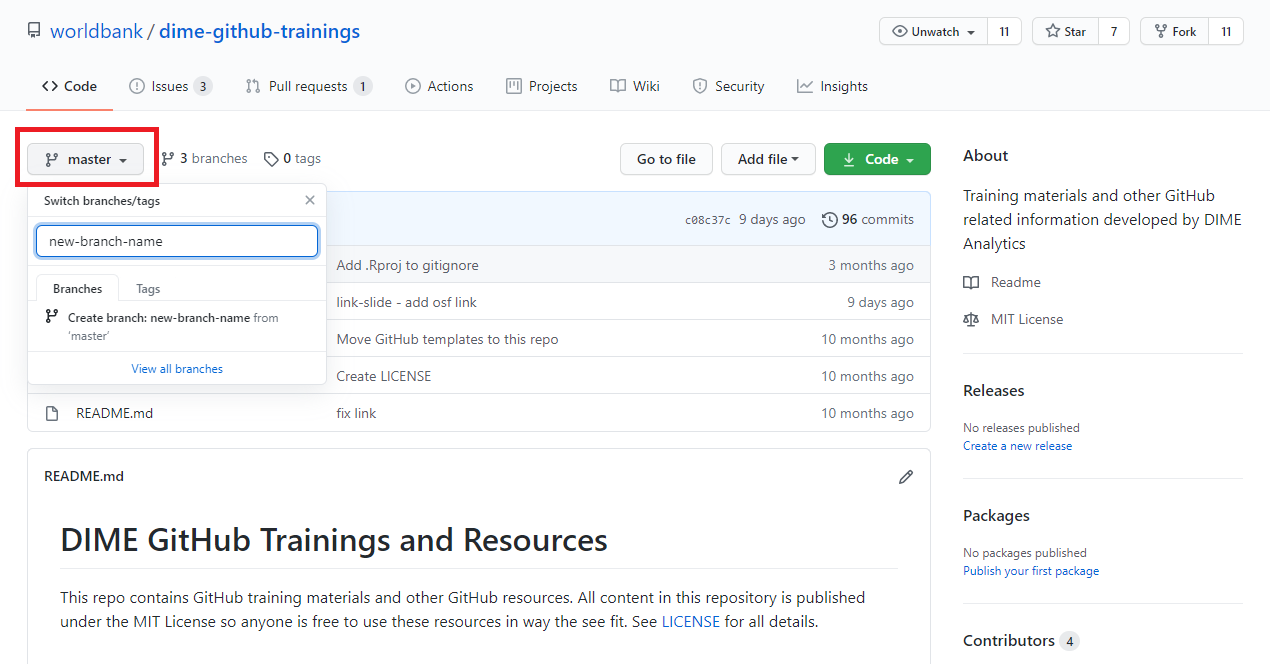
\includegraphics[width=.9\textwidth]{./img/new-branch-1.png}
\end{figure}
\end{frame}

\begin{frame}{Create branch on GitHub.com}
\begin{figure}
	\centering
	\includegraphics[width=.9\textwidth]{./img/new-branch-2.png}
\end{figure}
\end{frame}

\begin{frame}{Create branch on GitHub.com}
\begin{figure}
	\centering
	\includegraphics[width=.9\textwidth]{./img/new-branch-3.png}
\end{figure}
\hyperlink{Create a branch}{\beamerreturnbutton{contents page}}
\end{frame}

\end{document}
